\documentclass[reprint,amsmath,amssymb,showkeys,prd]{revtex4-2}

\usepackage{graphicx}
\usepackage{dcolumn}
\usepackage{bm}
\usepackage{hyperref}
% \usepackage{subcaption}
\usepackage[caption=false]{subfig}
\usepackage[mathlines]{lineno}
% \linenumbers\relax % Commence numbering lines

% \usepackage[showframe,%Uncomment any one of the following lines to test 
% scale=0.7, marginratio={1:1, 2:3}, ignoreall,% default settings
% text={7in,10in},centering,
% margin=1.5in,
% total={6.5in,8.75in}, top=1.2in, left=0.9in, includefoot,
% height=10in,a5paper,hmargin={3cm,0.8in},
% ]{geometry}

\begin{document}

\preprint{APS/123-QED}

\title{Periodictity of Two Fast Radio Bursts (FRB) Repeaters with Limited Detections: FRB20190915D and FRB20191106C}

\author{Murthadza Aznam}
\email{taza.aznam@gmail.com}
\author{Zamri Zainal Abidin}
% \email{zzaa@um.edu.my}
\author{Norsiah Hashim}
\author{Muhammad Hassan Zakie Yussoff}
\author{Matdhesh Kummar Jayaganthan}
\affiliation{
    Universiti Malaya, 50603 Kuala Lumpur, Wilayah Persekutuan Kuala Lumpur, Malaysia
}

\date{\today}

\begin{abstract}
Fast radio burst (FRB) is a class of transients characterized by its miliseconds scale duration with a relatively high dispersion measure. 
Some of them show repetition and among those, only some of them seem to repeat regularly.
This paper focuses on the characterization of the periodicity of FRBs whose repetition seems to be limited within a certain timeframe -- FRB20190915D and FRB20191106C as the chosen examples -- from a 3 year dataset provided by the CHIME/FRB.
This paper found that the periodicity can be characterized with more than 50\% certainty given that the waiting time is bimodally distributed despite the limited samples.

\end{abstract}

%\keywords{Suggested keywords}%Use showkeys class option if keyword
                              %display desired
\maketitle

\section{Introduction}

Fast Radio Burst (FRB) is a class of transients first discovered by \citet{lorimer_BrightMillisecondRadio_2007} with currently unknown origin.
It is characterized as a radio pulse with durations in the order of milliseconds and a relatively high dispersion measure.
Its high dispersion measure suggests an extragalactic origin consistent with observation of identified hosts such as in \citet{bannister_SingleFastRadio_2019, chatterjee_DirectLocalizationFast_2017, ravi_FastRadioBurst_2019}.

With increasing interests in FRBs, progress have been made in detections (especially with the commisioning of the CHIME/FRB telescope  \cite{thechimefrbcollaborationCHIMEFastRadio2018}  and in the future, BURSTT  \cite{lin_BURSTTBustlingUniverse_2022} ), theoretical models (a list of theories can be found in \citet{platts_LivingTheoryCatalogue_2019}), and analyses (especially on regularly repeating bursts such as FRB20121102A and FRB20180916B).
\citet{petroff_FastRadioBursts_2019} and their follow-up review, \citet{petroff_FastRadioBursts_2022}, summarizes the growth of FRB research in depth.

Currently, FRBs can be categorized as repeating or non-repeating.
The population seem to favor non-repeating FRBs over repeating FRBs as \cite{thechimefrbcollaborationCHIMEFastRadio2018} reports on 18 repeating sources (3.7 \%) are among 492 FRB sources detected\footnote{\url{https://www.chime-frb.ca/catalog}}.
A recent paper  \cite{andersen_CHIMEFRBDiscovery_2023}  estimates that repeating sources constitutes about 2.6 \% of known FRBs.
However, it is important to note that there is no guarantee that one-off FRBs will not repeat.
Following this assumption, the term `apparently non-repeating FRB' have been used in various papers, such as in \citet{cui_FastRadioBursts_2021, cui_StatisticalPropertiesFast_2021}; and \citet{katz_AbsencePeriodicityRepeating_2022}.

Multiple statistical analyses seem to support the idea that they are truly two different population of FRBs with consistent differences between repeating and non-repeating FRB in various properties \cite{cui_FastRadioBursts_2021, chen_OneoffRepeatingFast_2022, zhang_StatisticalSimilarityRepeating_2022} .
This consistency does not prevent some authors in assuming that a small part of the non-repeating FRBs might repeat in the future dubbed as `potentially repeating' or `repeater candidates', as was done by \citet{bohanchen_UncloakingHiddenRepeating_2021, luo_MachineLearningClassification_2022, zhu-ge_MachineLearningClassification_2022}; and \citet{pleunis_FastRadioBurst_2021}.

Regularly repeating FRBs such as FRB20121102A and FRB20180916B are rare.
Most of the repeaters currently identified has a limited sample which makes it hard to study its individual property.
As such, many repeaters are understudied as its low number of samples provide limited certainty.
Therefore, this paper intends to study the property of individual sources with limited samples.

Since periodicity generally requires many data points, this paper examines whether it is possible to determine the periodicity of a source with at least 50 \% confidence level using samples with more than 3 and less than 20 event counts.
If so, what are the criteria to differentiate between determinable and non-determinable periodicity?
Having this criteria can help to anticipate new detections.

\section{Methodology}

This paper will examine the periodicity of FRB20190915D (10 detections) and FRB20191106C (7 detections) from the CHIME/FRB Catalog 2023\footnote{\url{https://www.chime-frb.ca/repeater_catalog}}  \cite{andersen_CHIMEFRBDiscovery_2023}.
This paper will also include FRB20180916B (77 detections) from CHIME/FRB Catalog 1\footnotemark[1]\cite{thechimefrbcollaborationFirstCHIMEFRB2021}  to compare the validity of methods since its periodicity value is well quantified to be around 16 days \cite{thechimefrbcollaborationPeriodicActivityFast2020, sand_CHIMEFRBStudy_2023}.

\subsection{Periodogram}

A periodogram is a function of cost versus periods which quantifies the strength of the fit between the given period and the time series data.
The cost function depends on the method of choice.
The best period is chosen based on the period with the maximum or minimum cost.
While most periodogram methods choose the best period via the maximum cost, the phase dispersion minimization method chooses the minimum cost.
This section will describe the periodogram methods chosen for this paper.

\subsubsection{Method: Lomb--Scargle Periodogram (LS)}

The Lomb--Scargle periodogram \citet{lomb_LeastSquaresFrequencyAnalysis_1976, scargle_StudiesAstronomicalTime_1982} is the most commonly used in astronomy.
The cost function for this periodogram is the Fourier power which is to be maximized.
As such, it is a periodogram based on Fourier transform but it can also be approached as a least square optimization  \cite{vanderplas_UnderstandingLombScargle_2018} .
The widespread use of this method warrants its place in the `astropy` package\footnote{\url{https://docs.astropy.org/en/stable/api/astropy.timeseries.LombScargle.html}}, an astronomy package for the Python programming language.

\subsubsection{Method: Duty Cycle (DC)}

The Duty Cycle method is a phase--folding periodogram which measures the trial period with the longest continuous inactivity per cycle of a given FRB.
This method was introduced by \citet{rajwade_PossiblePeriodicActivity_2020} to measure the periodicity of FRB20121102A because of the nature of repeaters to be active within a certain period per cycle.
A duty cycle of 56 \% means that there is a continuous inactivity for 44 \% of the cycle.

\subsubsection{Method: Phase Dispersion Minimization (PDM)}

Phase Dispersion Minimization is a phase--folding method to determine the periodicity of non--sinusoidal time variation introduced by \citet{stellingwerf_PeriodDeterminationUsing_1978}. 
This method computes the variances, `theta', of the data with respect to mean light curve at each trial periods and minimizes it.
It is suitable for small dataset with irregularly sampled observations, such as the repeaters sampled in the CHIME/FRB 2023 Catalog.
This paper will use the Python wrapper of this algorithm written in C using the `py-pdm`\footnote{\url{https://github.com/ckm3/Py-PDM}} package.

\subsection{Parameter: Frequency Grid}

For this study, we chose a frequency grid of $f_\text{max} = 3^{-1} \text{days}^{-1}$ to $f_\text{min} = 0.5 * T_\text{obs}^{-1}\, \text{days}^{-1}$, where $T_\text{obs}$ is the length of observation (1,007 days).
The maximum frequency is set to $3^{-1} \text{days}^{-1}$ because if the period of FRBs is less than 3 days, we would see it much more often at a daily or bidaily rate.
On the other hand, the minimum frequency is chosen to minimize the windowing effect near the length of observation.
The number of frequencies in this frequency grid is adopted from \citet{vanderplas_UnderstandingLombScargle_2018} using the formula $N_\text{eval}=n_0T_\text{obs}f_\text{max}$ where $n_0$ is chosen to be 7.

\subsection{Uncertainty Estimation}

Periodograms do not usually have an associated uncertainty.
The level of confidence is treated on a case by case basis.
The Lomb--Scargle periodogram is equipped with a False Alarm Probability (FAP) associated at each power level to avoid false positives.
On the other hand, \citet{rajwade_PossiblePeriodicActivity_2020} approached the problem by calculating the full width at half maximum of the peak as their confidence region.

This paper estimates uncertainty by employing the leave-one-out strategy.
For each FRB repeaters, $k$ detections of the FRB repeaters are used to find the best period for the chosen periodogram method.
Then, for each detections, use $k-1$ sample detections through the same method -- each iteration removing a different detection.
Twich the standard deviation of the best periods from the $k$ samples of $k-1$ detections are used as the uncertainty.
The idea is that the uncertainty in the periodicity is tied to the fact that some observation might be missed.

\section{Result}

The results shown in Table \ref{tbl-result} accompanied by Figure \ref{fig-periodogram} for FRB20180916B using Lomb--Scargle and Duty Cycle methods are consistent with the periodicities from \citet{thechimefrbcollaborationPeriodicActivityFast2020} of 16.35±0.15 days and from \citet{sand_CHIMEFRBStudy_2023} of 16.34±0.07 days.
This consistency indicates that the methodology is reliable in determining periodicity using the available data.
The Phase Dispersion Minimization method, however, offshoots by about $\sim 1.4$ times the obtained periodicity from the previous two methods.

\begin{figure}[ht]
    \label{fig-periodogram}
    \caption{
    The periodograms of FRB20180916B (left), FRB20190915D (middle column) and FRB20191106C (right) using Lomb--Scargle method (top), Duty Cycle method (middle row) and Phase Dispersion Minimization (bottom).
    }
    \centering
    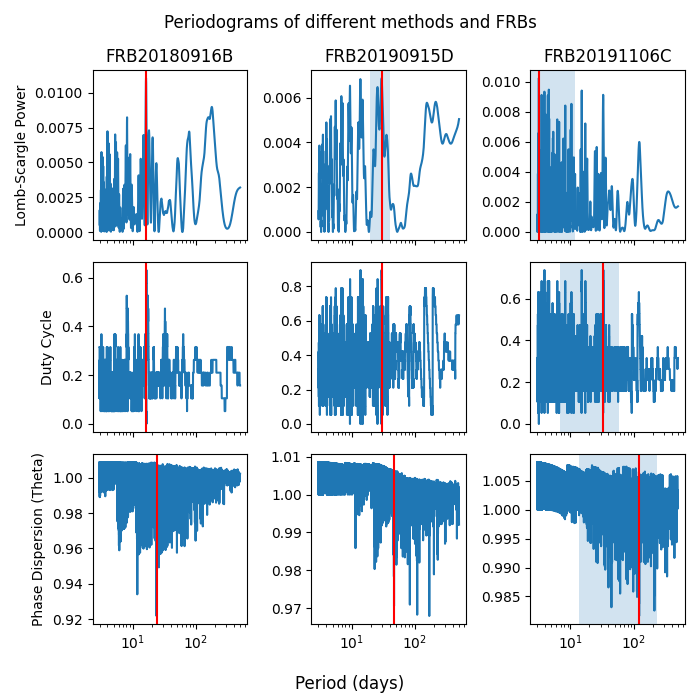
\includegraphics[width=0.5\textwidth]{periodograms.png}
\end{figure}

\begin{table}[!ht]
    \centering
    \caption{The periods obtained from the specified methods in days and its uncertainty. The percentage in brackets for the 'Duty Cycle' column is the active fraction of the cycle.}
    \begin{tabular}{l p{0.7in} p{0.7in} p{0.7in}}
    
    \hline
        \textbf{burst name} & \textbf{LS} & \textbf{DC} & \textbf{PDM} \\ \hline
        \textbf{FRB20180916B} & 16.33±0.00 & 16.30±0.21 (36.8 \%) & 23.56±0.00 \\ 
        \textbf{FRB20190915D} & 30.06±10.21 & 29.97±0.95 (10.5 \%) & 47.75±0.14 \\ 
        \textbf{FRB20191106C} & 3.16±8.80 & 33.16±26.21 (26.3 \%) & 122.31±108.51 \\ \hline
    \end{tabular}
    \label{tbl-result}
\end{table}

This pattern also emerges in the results for FRB20190915D with Lomb--Scargle and Duty Cycle methods showing a periodicity of 30.06±10.21 days and 29.97±0.95 days respectively, with Phase Dispersion Minimization offshooting to $1.5\sim 1.6$ times the two values.
This pattern indicates that the obtained values might point to the real periodicity of the newly discovered FRB20190915D even though the available data is limited.
The Phase Dispersion Minimization seems to consistently obtain $1.5 \times \text{period}$ days which is somewhat like a harmonic, equivalent to the second harmonic equivalent to $1.5\times \lambda$ standing wave. 

This is contrasted with the results for FRB20191106C.
It is apparent that FRB20191106C's periodicity is indeterminate because all three methods give different results.
This fact is supported by the large uncertainty region that accompanies the result. 

\begin{figure}[ht]
    \label{fig-fold}    
    \caption{Phase folded detection count of FRB at their selected periods. FRB20191106C is not included since the period is indeterminate.}
    \centering
        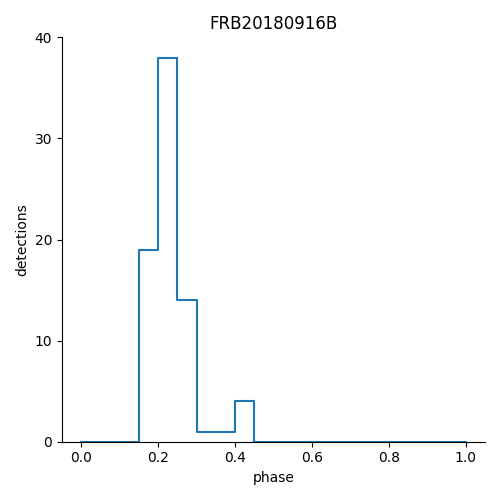
\includegraphics[width=0.23\textwidth]{FRB20180916B-phase-16.33.png}
        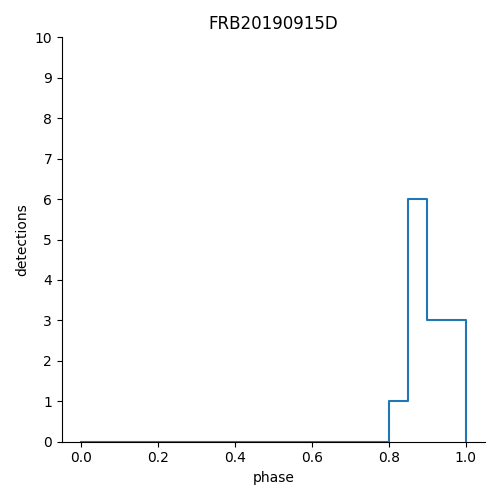
\includegraphics[width=0.23\textwidth]{FRB20190915D-phase-30.06.png}
\end{figure}

\section{Discussion}

\subsection{False Alarm Probability}

The False Alarm Probability (FAP) from the Lomb--Scargle periodogram can be used as a proxy of confidence level.
The FAP is computed using the `bootstrap' method implemented in astropy's `LombScargle' class.
It is found that each FRBs has a FAP of 13.3 \% (FRB20180916B), 57.0 \% (FRB20190915D) and 66.0 \% (FRB20191106C).
These values are consistent with the heuristics in the previous section that the value for FRB20180916B has a higher confidence than for FRB20190915D while values obtained for FRB20191106C has the least confidence.
The fact that the FAP for FRB20190915D is slightly above 50 \% but not any higher might be due to the fact that its detection only happens in a small time frame compared to the observation window.
Fixing the window to be between 20 Jun 2019 and 15 May 2020 reduces the FAP to 44.2 \% -- suggesting that there is more than 50 \% confidence level that it has a periodicity if treated as a time-limited event. 
Further discussion on this property is in Section \ref{sec-why-30}.

\subsection{Waiting time distribution}

\begin{figure}[h]
    \label{fig-waitingtime}
    \caption{The waiting time distribution of FRB20191106C, FRB20191106C, and FRB20190916B in the $\log_{10}$ scale.}
    \centering
    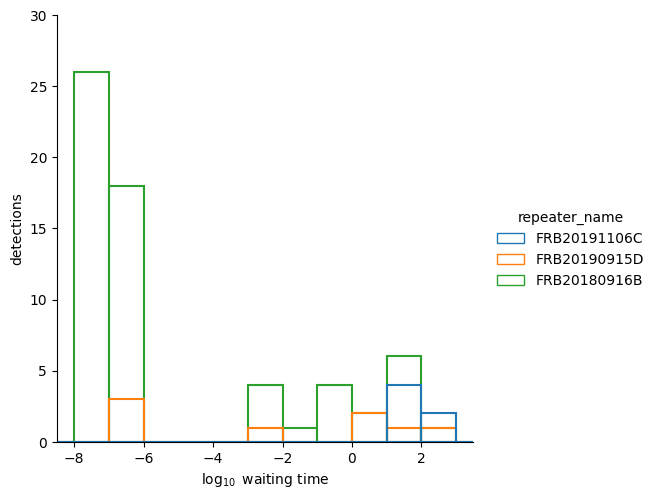
\includegraphics[width=0.5\textwidth]{waiting.png}
\end{figure}

One might wonder what distinguishes FRB20190915D from FRB20191106C which allowed one to have periodicity despite limited samples?
Looking at the waiting time distribution in \ref{fig-waitingtime}, FRB20190915D clearly shows bimodal distribution consistent with FRB20180916B (shown here) 
and FRB20121102A (shown in \citet{hewitt_AreciboObservationsBurst_2022} and \citet{jahns_FRB20121102ANovember_2022}).
Additionally, the waiting time of FRB20191106C is concentrated in the longer timescale compared to the bimodal distribution.
It seems that a bimodal distribution is required for an FRB to have a well-defined periodicity.


\subsection{Where is the rest of the detections?}\label{sec-why-30}

If it is indeed that FRB20190915D has a 30 day periodicity, why is there no additional detections within the 3 year window of the catalogue?
It might be the case that this FRB has a multi-term periodicity with this value representing it's short-term periodicity.
If that is the case, it's long-term periodicity is expected to be more than 2 years which is yet to be seen.
However, this is the same as hypothesizing that repeaters are possible repeaters with not-yet-observed repetition.

Another hypothesis that might explain this seemingly lack of regular detection is that FRB20190915D is a cataclysmic event with a periodic pulse and stopping at a certain point, such as the inspiraling of two magnetic bodies whose interaction releases some radio bursts.
This might explain the ever increasing detection count as it reaches peak and then no longer bursting.

\begin{figure}[ht]
    \label{fig-FRB20190915D-countplot}
    \caption{The number of detections per day of FRB20190915D between 20th Jun 2019 between 15th May 2020. The gray coloured regions indicate the active fractions (10 \%) in a 30 day cycle from 25th Jul 2018. Note that this graph focuses on this small timeframe because the datasets spans from 25th Jul 2018 to 26th Apr 2021 but is empty throughout the beginning and end for the specified FRB.}
    \centering
    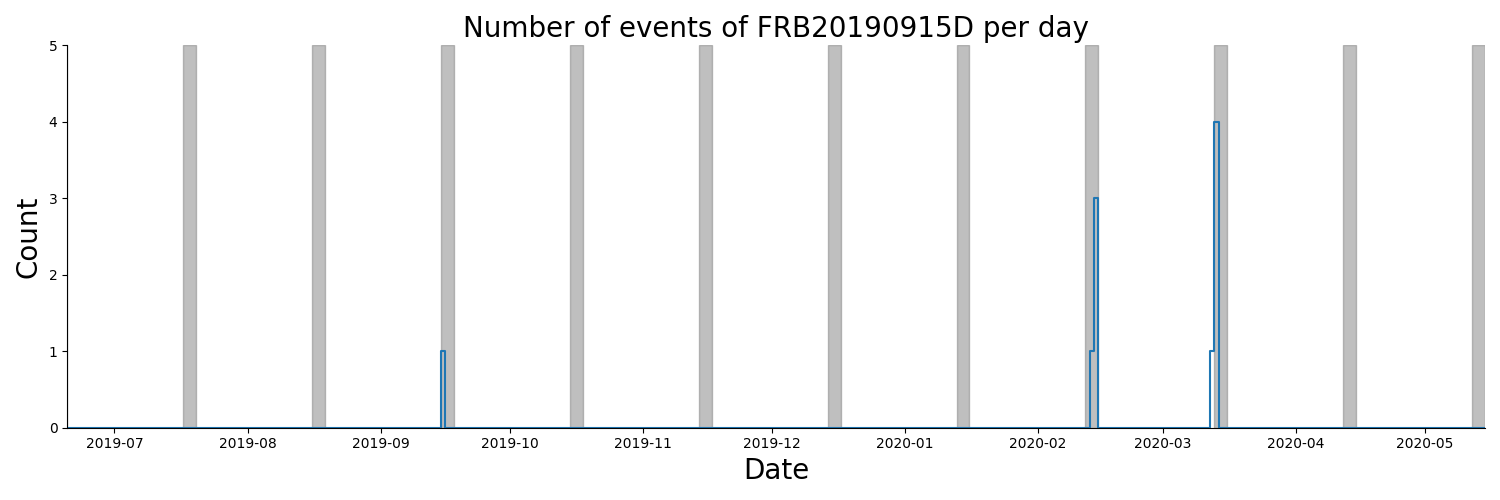
\includegraphics[width=0.5\textwidth]{./FRB20190915D-countplot.png}
\end{figure}

\section{Conclusion}

This paper determines that it is possible to evaluate the periodicity of FRBs despite small event counts.
The choice of periodogram seems to matter as the Phase Dispersion Minimization method seems to offshoot for FRBs, but using multiple periodogram methods help find a consistent pattern. 
The bimodal distribution of waiting times seems crucial in the determinability of its periodicity.
This paper also suggests that there might a new class of FRB whose repeatability seems limited -- such as an inspiraling collision -- suggesting that FRBs might be divided into three classes: (i) continuously repeating, (ii) limited repeating, or (iii) one-off.

\section{Acknowledgement}

The authors wishes to thank the team from CHIME/FRB for their initiative in open data which allowed this work to happen.
We would like to acknowledge the grant GPF081-2020 for funding the research activities of the radio cosmology lab group in Universiti Malaya in which the development of the Malaysian VGOS radio telescope is taking place.

\begin{thebibliography}{33}%
    \makeatletter
    \providecommand \@ifxundefined [1]{%
     \@ifx{#1\undefined}
    }%
    \providecommand \@ifnum [1]{%
     \ifnum #1\expandafter \@firstoftwo
     \else \expandafter \@secondoftwo
     \fi
    }%
    \providecommand \@ifx [1]{%
     \ifx #1\expandafter \@firstoftwo
     \else \expandafter \@secondoftwo
     \fi
    }%
    \providecommand \natexlab [1]{#1}%
    \providecommand \enquote  [1]{``#1''}%
    \providecommand \bibnamefont  [1]{#1}%
    \providecommand \bibfnamefont [1]{#1}%
    \providecommand \citenamefont [1]{#1}%
    \providecommand \href@noop [0]{\@secondoftwo}%
    \providecommand \href [0]{\begingroup \@sanitize@url \@href}%
    \providecommand \@href[1]{\@@startlink{#1}\@@href}%
    \providecommand \@@href[1]{\endgroup#1\@@endlink}%
    \providecommand \@sanitize@url [0]{\catcode `\\12\catcode `\$12\catcode `\&12\catcode `\#12\catcode `\^12\catcode `\_12\catcode `\%12\relax}%
    \providecommand \@@startlink[1]{}%
    \providecommand \@@endlink[0]{}%
    \providecommand \url  [0]{\begingroup\@sanitize@url \@url }%
    \providecommand \@url [1]{\endgroup\@href {#1}{\urlprefix }}%
    \providecommand \urlprefix  [0]{URL }%
    \providecommand \Eprint [0]{\href }%
    \providecommand \doibase [0]{https://doi.org/}%
    \providecommand \selectlanguage [0]{\@gobble}%
    \providecommand \bibinfo  [0]{\@secondoftwo}%
    \providecommand \bibfield  [0]{\@secondoftwo}%
    \providecommand \translation [1]{[#1]}%
    \providecommand \BibitemOpen [0]{}%
    \providecommand \bibitemStop [0]{}%
    \providecommand \bibitemNoStop [0]{.\EOS\space}%
    \providecommand \EOS [0]{\spacefactor3000\relax}%
    \providecommand \BibitemShut  [1]{\csname bibitem#1\endcsname}%
    \let\auto@bib@innerbib\@empty
    %</preamble>
    \bibitem [{\citenamefont {Lorimer}\ \emph {et~al.}(2007)\citenamefont {Lorimer}, \citenamefont {Bailes}, \citenamefont {McLaughlin}, \citenamefont {Narkevic},\ and\ \citenamefont {Crawford}}]{lorimer_BrightMillisecondRadio_2007}%
      \BibitemOpen
      \bibfield  {author} {\bibinfo {author} {\bibfnamefont {D.~R.}\ \bibnamefont {Lorimer}}, \bibinfo {author} {\bibfnamefont {M.}~\bibnamefont {Bailes}}, \bibinfo {author} {\bibfnamefont {M.~A.}\ \bibnamefont {McLaughlin}}, \bibinfo {author} {\bibfnamefont {D.~J.}\ \bibnamefont {Narkevic}},\ and\ \bibinfo {author} {\bibfnamefont {F.}~\bibnamefont {Crawford}},\ }\bibfield  {title} {\bibinfo {title} {A bright millisecond radio burst of extragalactic origin},\ }\href {https://doi.org/10.1126/science.1147532} {\bibfield  {journal} {\bibinfo  {journal} {Science}\ }\textbf {\bibinfo {volume} {318}},\ \bibinfo {pages} {777} (\bibinfo {year} {2007})},\ \Eprint {https://arxiv.org/abs/0709.4301} {arxiv:0709.4301 [astro-ph]} \BibitemShut {NoStop}%
    \bibitem [{\citenamefont {Bannister}\ \emph {et~al.}(2019)\citenamefont {Bannister}, \citenamefont {Deller}, \citenamefont {Phillips}, \citenamefont {Macquart}, \citenamefont {Prochaska}, \citenamefont {Tejos}, \citenamefont {Ryder}, \citenamefont {Sadler}, \citenamefont {Shannon}, \citenamefont {Simha}, \citenamefont {Day}, \citenamefont {McQuinn}, \citenamefont {{North-Hickey}}, \citenamefont {Bhandari}, \citenamefont {Arcus}, \citenamefont {Bennert}, \citenamefont {Burchett}, \citenamefont {Bouwhuis}, \citenamefont {Dodson}, \citenamefont {Ekers}, \citenamefont {Farah}, \citenamefont {Flynn}, \citenamefont {James}, \citenamefont {Kerr}, \citenamefont {Lenc}, \citenamefont {Mahony}, \citenamefont {O'Meara}, \citenamefont {Os{\l}owski}, \citenamefont {Qiu}, \citenamefont {Treu}, \citenamefont {U}, \citenamefont {Bateman}, \citenamefont {Bock}, \citenamefont {Bolton}, \citenamefont {Brown}, \citenamefont {Bunton}, \citenamefont {Chippendale}, \citenamefont {Cooray}, \citenamefont {Cornwell}, \citenamefont {Gupta}, \citenamefont {Hayman}, \citenamefont {Kesteven}, \citenamefont {Koribalski}, \citenamefont {MacLeod}, \citenamefont {{McClure-Griffiths}}, \citenamefont {Neuhold}, \citenamefont {Norris}, \citenamefont {Pilawa}, \citenamefont {Qiao}, \citenamefont {Reynolds}, \citenamefont {Roxby}, \citenamefont {Shimwell}, \citenamefont {Voronkov},\ and\ \citenamefont {Wilson}}]{bannister_SingleFastRadio_2019}%
      \BibitemOpen
      \bibfield  {author} {\bibinfo {author} {\bibfnamefont {K.~W.}\ \bibnamefont {Bannister}}, \bibinfo {author} {\bibfnamefont {A.~T.}\ \bibnamefont {Deller}}, \bibinfo {author} {\bibfnamefont {C.}~\bibnamefont {Phillips}}, \bibinfo {author} {\bibfnamefont {J.~P.}\ \bibnamefont {Macquart}}, \bibinfo {author} {\bibfnamefont {J.~X.}\ \bibnamefont {Prochaska}}, \bibinfo {author} {\bibfnamefont {N.}~\bibnamefont {Tejos}}, \bibinfo {author} {\bibfnamefont {S.~D.}\ \bibnamefont {Ryder}}, \bibinfo {author} {\bibfnamefont {E.~M.}\ \bibnamefont {Sadler}}, \bibinfo {author} {\bibfnamefont {R.~M.}\ \bibnamefont {Shannon}}, \bibinfo {author} {\bibfnamefont {S.}~\bibnamefont {Simha}}, \bibinfo {author} {\bibfnamefont {C.~K.}\ \bibnamefont {Day}}, \bibinfo {author} {\bibfnamefont {M.}~\bibnamefont {McQuinn}}, \bibinfo {author} {\bibfnamefont {F.~O.}\ \bibnamefont {{North-Hickey}}}, \bibinfo {author} {\bibfnamefont {S.}~\bibnamefont {Bhandari}}, \bibinfo {author} {\bibfnamefont {W.~R.}\ \bibnamefont {Arcus}}, \bibinfo {author} {\bibfnamefont {V.~N.}\ \bibnamefont {Bennert}}, \bibinfo {author} {\bibfnamefont {J.}~\bibnamefont {Burchett}}, \bibinfo {author} {\bibfnamefont {M.}~\bibnamefont {Bouwhuis}}, \bibinfo {author} {\bibfnamefont {R.}~\bibnamefont {Dodson}}, \bibinfo {author} {\bibfnamefont {R.~D.}\ \bibnamefont {Ekers}}, \bibinfo {author} {\bibfnamefont {W.}~\bibnamefont {Farah}}, \bibinfo {author} {\bibfnamefont {C.}~\bibnamefont {Flynn}}, \bibinfo {author} {\bibfnamefont {C.~W.}\ \bibnamefont {James}}, \bibinfo {author} {\bibfnamefont {M.}~\bibnamefont {Kerr}}, \bibinfo {author} {\bibfnamefont {E.}~\bibnamefont {Lenc}}, \bibinfo {author} {\bibfnamefont {E.~K.}\ \bibnamefont {Mahony}}, \bibinfo {author} {\bibfnamefont {J.}~\bibnamefont {O'Meara}}, \bibinfo {author} {\bibfnamefont {S.}~\bibnamefont {Os{\l}owski}}, \bibinfo {author} {\bibfnamefont {H.}~\bibnamefont {Qiu}}, \bibinfo {author} {\bibfnamefont {T.}~\bibnamefont {Treu}}, \bibinfo {author} {\bibfnamefont {V.}~\bibnamefont {U}}, \bibinfo {author} {\bibfnamefont {T.~J.}\ \bibnamefont {Bateman}}, \bibinfo {author} {\bibfnamefont {D.~C.~J.}\ \bibnamefont {Bock}}, \bibinfo {author} {\bibfnamefont {R.~J.}\ \bibnamefont {Bolton}}, \bibinfo {author} {\bibfnamefont {A.}~\bibnamefont {Brown}}, \bibinfo {author} {\bibfnamefont {J.~D.}\ \bibnamefont {Bunton}}, \bibinfo {author} {\bibfnamefont {A.~P.}\ \bibnamefont {Chippendale}}, \bibinfo {author} {\bibfnamefont {F.~R.}\ \bibnamefont {Cooray}}, \bibinfo {author} {\bibfnamefont {T.}~\bibnamefont {Cornwell}}, \bibinfo {author} {\bibfnamefont {N.}~\bibnamefont {Gupta}}, \bibinfo {author} {\bibfnamefont {D.~B.}\ \bibnamefont {Hayman}}, \bibinfo {author} {\bibfnamefont {M.}~\bibnamefont {Kesteven}}, \bibinfo {author} {\bibfnamefont {B.~S.}\ \bibnamefont {Koribalski}}, \bibinfo {author} {\bibfnamefont {A.}~\bibnamefont {MacLeod}}, \bibinfo {author} {\bibfnamefont {N.~M.}\ \bibnamefont {{McClure-Griffiths}}}, \bibinfo {author} {\bibfnamefont {S.}~\bibnamefont {Neuhold}}, \bibinfo {author} {\bibfnamefont {R.~P.}\ \bibnamefont {Norris}}, \bibinfo {author} {\bibfnamefont {M.~A.}\ \bibnamefont {Pilawa}}, \bibinfo {author} {\bibfnamefont {R.~Y.}\ \bibnamefont {Qiao}}, \bibinfo {author} {\bibfnamefont {J.}~\bibnamefont {Reynolds}}, \bibinfo {author} {\bibfnamefont {D.~N.}\ \bibnamefont {Roxby}}, \bibinfo {author} {\bibfnamefont {T.~W.}\ \bibnamefont {Shimwell}}, \bibinfo {author} {\bibfnamefont {M.~A.}\ \bibnamefont {Voronkov}},\ and\ \bibinfo {author} {\bibfnamefont {C.~D.}\ \bibnamefont {Wilson}},\ }\bibfield  {title} {\bibinfo {title} {A single fast radio burst localized to a massive galaxy at cosmological distance},\ }\href {https://doi.org/10.1126/science.aaw5903} {\bibfield  {journal} {\bibinfo  {journal} {Science}\ }\textbf {\bibinfo {volume} {365}},\ \bibinfo {pages} {565} (\bibinfo {year} {2019})}\BibitemShut {NoStop}%
    \bibitem [{\citenamefont {Chatterjee}\ \emph {et~al.}(2017)\citenamefont {Chatterjee}, \citenamefont {Law}, \citenamefont {Wharton}, \citenamefont {{Burke-Spolaor}}, \citenamefont {Hessels}, \citenamefont {Bower}, \citenamefont {Cordes}, \citenamefont {Tendulkar}, \citenamefont {Bassa}, \citenamefont {Demorest}, \citenamefont {Butler}, \citenamefont {Seymour}, \citenamefont {Scholz}, \citenamefont {Abruzzo}, \citenamefont {Bogdanov}, \citenamefont {Kaspi}, \citenamefont {Keimpema}, \citenamefont {Lazio}, \citenamefont {Marcote}, \citenamefont {McLaughlin}, \citenamefont {Paragi}, \citenamefont {Ransom}, \citenamefont {Rupen}, \citenamefont {Spitler},\ and\ \citenamefont {{van Langevelde}}}]{chatterjee_DirectLocalizationFast_2017}%
      \BibitemOpen
      \bibfield  {author} {\bibinfo {author} {\bibfnamefont {S.}~\bibnamefont {Chatterjee}}, \bibinfo {author} {\bibfnamefont {C.~J.}\ \bibnamefont {Law}}, \bibinfo {author} {\bibfnamefont {R.~S.}\ \bibnamefont {Wharton}}, \bibinfo {author} {\bibfnamefont {S.}~\bibnamefont {{Burke-Spolaor}}}, \bibinfo {author} {\bibfnamefont {J.~W.~T.}\ \bibnamefont {Hessels}}, \bibinfo {author} {\bibfnamefont {G.~C.}\ \bibnamefont {Bower}}, \bibinfo {author} {\bibfnamefont {J.~M.}\ \bibnamefont {Cordes}}, \bibinfo {author} {\bibfnamefont {S.~P.}\ \bibnamefont {Tendulkar}}, \bibinfo {author} {\bibfnamefont {C.~G.}\ \bibnamefont {Bassa}}, \bibinfo {author} {\bibfnamefont {P.}~\bibnamefont {Demorest}}, \bibinfo {author} {\bibfnamefont {B.~J.}\ \bibnamefont {Butler}}, \bibinfo {author} {\bibfnamefont {A.}~\bibnamefont {Seymour}}, \bibinfo {author} {\bibfnamefont {P.}~\bibnamefont {Scholz}}, \bibinfo {author} {\bibfnamefont {M.~W.}\ \bibnamefont {Abruzzo}}, \bibinfo {author} {\bibfnamefont {S.}~\bibnamefont {Bogdanov}}, \bibinfo {author} {\bibfnamefont {V.~M.}\ \bibnamefont {Kaspi}}, \bibinfo {author} {\bibfnamefont {A.}~\bibnamefont {Keimpema}}, \bibinfo {author} {\bibfnamefont {T.~J.~W.}\ \bibnamefont {Lazio}}, \bibinfo {author} {\bibfnamefont {B.}~\bibnamefont {Marcote}}, \bibinfo {author} {\bibfnamefont {M.~A.}\ \bibnamefont {McLaughlin}}, \bibinfo {author} {\bibfnamefont {Z.}~\bibnamefont {Paragi}}, \bibinfo {author} {\bibfnamefont {S.~M.}\ \bibnamefont {Ransom}}, \bibinfo {author} {\bibfnamefont {M.}~\bibnamefont {Rupen}}, \bibinfo {author} {\bibfnamefont {L.~G.}\ \bibnamefont {Spitler}},\ and\ \bibinfo {author} {\bibfnamefont {H.~J.}\ \bibnamefont {{van Langevelde}}},\ }\bibfield  {title} {\bibinfo {title} {A direct localization of a fast radio burst and its host},\ }\href {https://doi.org/10.1038/nature20797} {\bibfield  {journal} {\bibinfo  {journal} {Nature}\ }\textbf {\bibinfo {volume} {541}},\ \bibinfo {pages} {58} (\bibinfo {year} {2017})}\BibitemShut {NoStop}%
    \bibitem [{\citenamefont {Ravi}\ \emph {et~al.}(2019)\citenamefont {Ravi}, \citenamefont {Catha}, \citenamefont {D'Addario}, \citenamefont {Djorgovski}, \citenamefont {Hallinan}, \citenamefont {Hobbs}, \citenamefont {Kocz}, \citenamefont {Kulkarni}, \citenamefont {Shi}, \citenamefont {Vedantham}, \citenamefont {Weinreb},\ and\ \citenamefont {Woody}}]{ravi_FastRadioBurst_2019}%
      \BibitemOpen
      \bibfield  {author} {\bibinfo {author} {\bibfnamefont {V.}~\bibnamefont {Ravi}}, \bibinfo {author} {\bibfnamefont {M.}~\bibnamefont {Catha}}, \bibinfo {author} {\bibfnamefont {L.}~\bibnamefont {D'Addario}}, \bibinfo {author} {\bibfnamefont {S.~G.}\ \bibnamefont {Djorgovski}}, \bibinfo {author} {\bibfnamefont {G.}~\bibnamefont {Hallinan}}, \bibinfo {author} {\bibfnamefont {R.}~\bibnamefont {Hobbs}}, \bibinfo {author} {\bibfnamefont {J.}~\bibnamefont {Kocz}}, \bibinfo {author} {\bibfnamefont {S.~R.}\ \bibnamefont {Kulkarni}}, \bibinfo {author} {\bibfnamefont {J.}~\bibnamefont {Shi}}, \bibinfo {author} {\bibfnamefont {H.~K.}\ \bibnamefont {Vedantham}}, \bibinfo {author} {\bibfnamefont {S.}~\bibnamefont {Weinreb}},\ and\ \bibinfo {author} {\bibfnamefont {D.~P.}\ \bibnamefont {Woody}},\ }\bibfield  {title} {\bibinfo {title} {A fast radio burst localized to a massive galaxy},\ }\href {https://doi.org/10.1038/s41586-019-1389-7} {\bibfield  {journal} {\bibinfo  {journal} {Nature}\ }\textbf {\bibinfo {volume} {572}},\ \bibinfo {pages} {352} (\bibinfo {year} {2019})}\BibitemShut {NoStop}%
    \bibitem [{\citenamefont {{The CHIME/FRB Collaboration}}\ \emph {et~al.}(2018)\citenamefont {{The CHIME/FRB Collaboration}}, \citenamefont {Amiri}, \citenamefont {Bandura}, \citenamefont {Berger}, \citenamefont {Bhardwaj}, \citenamefont {Boyce}, \citenamefont {Boyle}, \citenamefont {Brar}, \citenamefont {Burhanpurkar}, \citenamefont {Chawla}, \citenamefont {Chowdhury}, \citenamefont {Cliche}, \citenamefont {Cranmer}, \citenamefont {Cubranic}, \citenamefont {Deng}, \citenamefont {Denman}, \citenamefont {Dobbs}, \citenamefont {Fandino}, \citenamefont {Fonseca}, \citenamefont {Gaensler}, \citenamefont {Giri}, \citenamefont {Gilbert}, \citenamefont {Good}, \citenamefont {Guliani}, \citenamefont {Halpern}, \citenamefont {Hinshaw}, \citenamefont {Hofer}, \citenamefont {Josephy}, \citenamefont {Kaspi}, \citenamefont {Landecker}, \citenamefont {Lang}, \citenamefont {Liao}, \citenamefont {Masui}, \citenamefont {{Mena-Parra}}, \citenamefont {Naidu}, \citenamefont {Newburgh}, \citenamefont {Ng}, \citenamefont {Patel}, \citenamefont {Pen}, \citenamefont {{Pinsonneault-Marotte}}, \citenamefont {Pleunis}, \citenamefont {Ravandi}, \citenamefont {Ransom}, \citenamefont {Renard}, \citenamefont {Scholz}, \citenamefont {Sigurdson}, \citenamefont {Siegel}, \citenamefont {Smith}, \citenamefont {Stairs}, \citenamefont {Tendulkar}, \citenamefont {Vanderlinde},\ and\ \citenamefont {Wiebe}}]{thechimefrbcollaborationCHIMEFastRadio2018}%
      \BibitemOpen
      \bibfield  {author} {\bibinfo {author} {\bibnamefont {{The CHIME/FRB Collaboration}}}, \bibinfo {author} {\bibfnamefont {M.}~\bibnamefont {Amiri}}, \bibinfo {author} {\bibfnamefont {K.}~\bibnamefont {Bandura}}, \bibinfo {author} {\bibfnamefont {P.}~\bibnamefont {Berger}}, \bibinfo {author} {\bibfnamefont {M.}~\bibnamefont {Bhardwaj}}, \bibinfo {author} {\bibfnamefont {M.~M.}\ \bibnamefont {Boyce}}, \bibinfo {author} {\bibfnamefont {P.~J.}\ \bibnamefont {Boyle}}, \bibinfo {author} {\bibfnamefont {C.}~\bibnamefont {Brar}}, \bibinfo {author} {\bibfnamefont {M.}~\bibnamefont {Burhanpurkar}}, \bibinfo {author} {\bibfnamefont {P.}~\bibnamefont {Chawla}}, \bibinfo {author} {\bibfnamefont {J.}~\bibnamefont {Chowdhury}}, \bibinfo {author} {\bibfnamefont {J.~F.}\ \bibnamefont {Cliche}}, \bibinfo {author} {\bibfnamefont {M.~D.}\ \bibnamefont {Cranmer}}, \bibinfo {author} {\bibfnamefont {D.}~\bibnamefont {Cubranic}}, \bibinfo {author} {\bibfnamefont {M.}~\bibnamefont {Deng}}, \bibinfo {author} {\bibfnamefont {N.}~\bibnamefont {Denman}}, \bibinfo {author} {\bibfnamefont {M.}~\bibnamefont {Dobbs}}, \bibinfo {author} {\bibfnamefont {M.}~\bibnamefont {Fandino}}, \bibinfo {author} {\bibfnamefont {E.}~\bibnamefont {Fonseca}}, \bibinfo {author} {\bibfnamefont {B.~M.}\ \bibnamefont {Gaensler}}, \bibinfo {author} {\bibfnamefont {U.}~\bibnamefont {Giri}}, \bibinfo {author} {\bibfnamefont {A.~J.}\ \bibnamefont {Gilbert}}, \bibinfo {author} {\bibfnamefont {D.~C.}\ \bibnamefont {Good}}, \bibinfo {author} {\bibfnamefont {S.}~\bibnamefont {Guliani}}, \bibinfo {author} {\bibfnamefont {M.}~\bibnamefont {Halpern}}, \bibinfo {author} {\bibfnamefont {G.}~\bibnamefont {Hinshaw}}, \bibinfo {author} {\bibfnamefont {C.}~\bibnamefont {Hofer}}, \bibinfo {author} {\bibfnamefont {A.}~\bibnamefont {Josephy}}, \bibinfo {author} {\bibfnamefont {V.~M.}\ \bibnamefont {Kaspi}}, \bibinfo {author} {\bibfnamefont {T.~L.}\ \bibnamefont {Landecker}}, \bibinfo {author} {\bibfnamefont {D.}~\bibnamefont {Lang}}, \bibinfo {author} {\bibfnamefont {H.}~\bibnamefont {Liao}}, \bibinfo {author} {\bibfnamefont {K.~W.}\ \bibnamefont {Masui}}, \bibinfo {author} {\bibfnamefont {J.}~\bibnamefont {{Mena-Parra}}}, \bibinfo {author} {\bibfnamefont {A.}~\bibnamefont {Naidu}}, \bibinfo {author} {\bibfnamefont {L.~B.}\ \bibnamefont {Newburgh}}, \bibinfo {author} {\bibfnamefont {C.}~\bibnamefont {Ng}}, \bibinfo {author} {\bibfnamefont {C.}~\bibnamefont {Patel}}, \bibinfo {author} {\bibfnamefont {U.-L.}\ \bibnamefont {Pen}}, \bibinfo {author} {\bibfnamefont {T.}~\bibnamefont {{Pinsonneault-Marotte}}}, \bibinfo {author} {\bibfnamefont {Z.}~\bibnamefont {Pleunis}}, \bibinfo {author} {\bibfnamefont {M.~R.}\ \bibnamefont {Ravandi}}, \bibinfo {author} {\bibfnamefont {S.~M.}\ \bibnamefont {Ransom}}, \bibinfo {author} {\bibfnamefont {A.}~\bibnamefont {Renard}}, \bibinfo {author} {\bibfnamefont {P.}~\bibnamefont {Scholz}}, \bibinfo {author} {\bibfnamefont {K.}~\bibnamefont {Sigurdson}}, \bibinfo {author} {\bibfnamefont {S.~R.}\ \bibnamefont {Siegel}}, \bibinfo {author} {\bibfnamefont {K.~M.}\ \bibnamefont {Smith}}, \bibinfo {author} {\bibfnamefont {I.~H.}\ \bibnamefont {Stairs}}, \bibinfo {author} {\bibfnamefont {S.~P.}\ \bibnamefont {Tendulkar}}, \bibinfo {author} {\bibfnamefont {K.}~\bibnamefont {Vanderlinde}},\ and\ \bibinfo {author} {\bibfnamefont {D.~V.}\ \bibnamefont {Wiebe}},\ }\bibfield  {title} {\bibinfo {title} {The {{CHIME Fast Radio Burst Project}}: {{System Overview}}},\ }\href {https://doi.org/10.3847/1538-4357/aad188} {\bibfield  {journal} {\bibinfo  {journal} {The Astrophysical Journal}\ }\textbf {\bibinfo {volume} {863}},\ \bibinfo {pages} {48} (\bibinfo {year} {2018})},\ \Eprint {https://arxiv.org/abs/1803.11235} {arxiv:1803.11235 [astro-ph]} \BibitemShut {NoStop}%
    \bibitem [{\citenamefont {Lin}\ \emph {et~al.}(2022)\citenamefont {Lin}, \citenamefont {Lin}, \citenamefont {Li}, \citenamefont {Tseng}, \citenamefont {Jiang}, \citenamefont {Wang}, \citenamefont {Cheng}, \citenamefont {Pen}, \citenamefont {Chen}, \citenamefont {Chen}, \citenamefont {Chen}, \citenamefont {Goto}, \citenamefont {Hashimoto}, \citenamefont {Hwang}, \citenamefont {King}, \citenamefont {Kubo}, \citenamefont {Kuo}, \citenamefont {Mills}, \citenamefont {Nam}, \citenamefont {Oshiro}, \citenamefont {Shen}, \citenamefont {Tseng}, \citenamefont {Wang}, \citenamefont {Wu}, \citenamefont {Bower}, \citenamefont {Chang}, \citenamefont {Chen}, \citenamefont {Chen}, \citenamefont {Chiang}, \citenamefont {Fedynitch}, \citenamefont {Gusinskaia}, \citenamefont {Ho}, \citenamefont {Hsiao}, \citenamefont {Hu}, \citenamefont {Huang}, \citenamefont {J{\'a}uregui~Garc{\'i}a}, \citenamefont {Kim}, \citenamefont {Kuo}, \citenamefont {Ling}, \citenamefont {On}, \citenamefont {Peterson}, \citenamefont {R.~Raquel}, \citenamefont {Su}, \citenamefont {Uno}, \citenamefont {Wu}, \citenamefont {Yamasaki},\ and\ \citenamefont {Zhu}}]{lin_BURSTTBustlingUniverse_2022}%
      \BibitemOpen
      \bibfield  {author} {\bibinfo {author} {\bibfnamefont {H.-H.}\ \bibnamefont {Lin}}, \bibinfo {author} {\bibfnamefont {K.-y.}\ \bibnamefont {Lin}}, \bibinfo {author} {\bibfnamefont {C.-T.}\ \bibnamefont {Li}}, \bibinfo {author} {\bibfnamefont {Y.-H.}\ \bibnamefont {Tseng}}, \bibinfo {author} {\bibfnamefont {H.}~\bibnamefont {Jiang}}, \bibinfo {author} {\bibfnamefont {J.-H.}\ \bibnamefont {Wang}}, \bibinfo {author} {\bibfnamefont {J.-C.}\ \bibnamefont {Cheng}}, \bibinfo {author} {\bibfnamefont {U.-L.}\ \bibnamefont {Pen}}, \bibinfo {author} {\bibfnamefont {M.-T.}\ \bibnamefont {Chen}}, \bibinfo {author} {\bibfnamefont {P.}~\bibnamefont {Chen}}, \bibinfo {author} {\bibfnamefont {Y.}~\bibnamefont {Chen}}, \bibinfo {author} {\bibfnamefont {T.}~\bibnamefont {Goto}}, \bibinfo {author} {\bibfnamefont {T.}~\bibnamefont {Hashimoto}}, \bibinfo {author} {\bibfnamefont {Y.-J.}\ \bibnamefont {Hwang}}, \bibinfo {author} {\bibfnamefont {S.-K.}\ \bibnamefont {King}}, \bibinfo {author} {\bibfnamefont {D.}~\bibnamefont {Kubo}}, \bibinfo {author} {\bibfnamefont {C.-Y.}\ \bibnamefont {Kuo}}, \bibinfo {author} {\bibfnamefont {A.}~\bibnamefont {Mills}}, \bibinfo {author} {\bibfnamefont {J.}~\bibnamefont {Nam}}, \bibinfo {author} {\bibfnamefont {P.}~\bibnamefont {Oshiro}}, \bibinfo {author} {\bibfnamefont {C.-S.}\ \bibnamefont {Shen}}, \bibinfo {author} {\bibfnamefont {H.-C.}\ \bibnamefont {Tseng}}, \bibinfo {author} {\bibfnamefont {S.-H.}\ \bibnamefont {Wang}}, \bibinfo {author} {\bibfnamefont {V.~F.-S.}\ \bibnamefont {Wu}}, \bibinfo {author} {\bibfnamefont {G.}~\bibnamefont {Bower}}, \bibinfo {author} {\bibfnamefont {S.-H.}\ \bibnamefont {Chang}}, \bibinfo {author} {\bibfnamefont {P.-A.}\ \bibnamefont {Chen}}, \bibinfo {author} {\bibfnamefont {Y.-C.}\ \bibnamefont {Chen}}, \bibinfo {author} {\bibfnamefont {Y.-K.}\ \bibnamefont {Chiang}}, \bibinfo {author} {\bibfnamefont {A.}~\bibnamefont {Fedynitch}}, \bibinfo {author} {\bibfnamefont {N.}~\bibnamefont {Gusinskaia}}, \bibinfo {author} {\bibfnamefont {S.~C.~C.}\ \bibnamefont {Ho}}, \bibinfo {author} {\bibfnamefont {T.~Y.~Y.}\ \bibnamefont {Hsiao}}, \bibinfo {author} {\bibfnamefont {C.-P.}\ \bibnamefont {Hu}}, \bibinfo {author} {\bibfnamefont {Y.~D.}\ \bibnamefont {Huang}}, \bibinfo {author} {\bibfnamefont {J.~M.}\ \bibnamefont {J{\'a}uregui~Garc{\'i}a}}, \bibinfo {author} {\bibfnamefont {S.~J.}\ \bibnamefont {Kim}}, \bibinfo {author} {\bibfnamefont {C.-Y.}\ \bibnamefont {Kuo}}, \bibinfo {author} {\bibfnamefont {D.~F.-J.}\ \bibnamefont {Ling}}, \bibinfo {author} {\bibfnamefont {A.~Y.~L.}\ \bibnamefont {On}}, \bibinfo {author} {\bibfnamefont {J.~B.}\ \bibnamefont {Peterson}}, \bibinfo {author} {\bibfnamefont {B.~J.}\ \bibnamefont {R.~Raquel}}, \bibinfo {author} {\bibfnamefont {S.-C.}\ \bibnamefont {Su}}, \bibinfo {author} {\bibfnamefont {Y.}~\bibnamefont {Uno}}, \bibinfo {author} {\bibfnamefont {C.~K.~W.}\ \bibnamefont {Wu}}, \bibinfo {author} {\bibfnamefont {S.}~\bibnamefont {Yamasaki}},\ and\ \bibinfo {author} {\bibfnamefont {H.-M.}\ \bibnamefont {Zhu}},\ }\bibfield  {title} {\bibinfo {title} {{{BURSTT}}: {{Bustling Universe Radio Survey Telescope}} in {{Taiwan}}},\ }\href {https://doi.org/10.1088/1538-3873/ac8f71} {\bibfield  {journal} {\bibinfo  {journal} {Publications of the Astronomical Society of the Pacific}\ }\textbf {\bibinfo {volume} {134}},\ \bibinfo {pages} {094106} (\bibinfo {year} {2022})}\BibitemShut {NoStop}%
    \bibitem [{\citenamefont {Platts}\ \emph {et~al.}(2019)\citenamefont {Platts}, \citenamefont {Weltman}, \citenamefont {Walters}, \citenamefont {Tendulkar}, \citenamefont {Gordin},\ and\ \citenamefont {Kandhai}}]{platts_LivingTheoryCatalogue_2019}%
      \BibitemOpen
      \bibfield  {author} {\bibinfo {author} {\bibfnamefont {E.}~\bibnamefont {Platts}}, \bibinfo {author} {\bibfnamefont {A.}~\bibnamefont {Weltman}}, \bibinfo {author} {\bibfnamefont {A.}~\bibnamefont {Walters}}, \bibinfo {author} {\bibfnamefont {S.~P.}\ \bibnamefont {Tendulkar}}, \bibinfo {author} {\bibfnamefont {J.~E.~B.}\ \bibnamefont {Gordin}},\ and\ \bibinfo {author} {\bibfnamefont {S.}~\bibnamefont {Kandhai}},\ }\bibfield  {title} {\bibinfo {title} {A {{Living Theory Catalogue}} for {{Fast Radio Bursts}}},\ }\href {https://doi.org/10.1016/j.physrep.2019.06.003} {\bibfield  {journal} {\bibinfo  {journal} {Physics Reports}\ }\textbf {\bibinfo {volume} {821}},\ \bibinfo {pages} {1} (\bibinfo {year} {2019})},\ \Eprint {https://arxiv.org/abs/1810.05836} {arxiv:1810.05836 [astro-ph]} \BibitemShut {NoStop}%
    \bibitem [{\citenamefont {Petroff}\ \emph {et~al.}(2019)\citenamefont {Petroff}, \citenamefont {Hessels},\ and\ \citenamefont {Lorimer}}]{petroff_FastRadioBursts_2019}%
      \BibitemOpen
      \bibfield  {author} {\bibinfo {author} {\bibfnamefont {E.}~\bibnamefont {Petroff}}, \bibinfo {author} {\bibfnamefont {J.~W.~T.}\ \bibnamefont {Hessels}},\ and\ \bibinfo {author} {\bibfnamefont {D.~R.}\ \bibnamefont {Lorimer}},\ }\bibfield  {title} {\bibinfo {title} {Fast radio bursts},\ }\href {https://doi.org/10.1007/s00159-019-0116-6} {\bibfield  {journal} {\bibinfo  {journal} {The Astronomy and Astrophysics Review}\ }\textbf {\bibinfo {volume} {27}},\ \bibinfo {pages} {75} (\bibinfo {year} {2019})}\BibitemShut {NoStop}%
    \bibitem [{\citenamefont {Petroff}\ \emph {et~al.}(2022)\citenamefont {Petroff}, \citenamefont {Hessels},\ and\ \citenamefont {Lorimer}}]{petroff_FastRadioBursts_2022}%
      \BibitemOpen
      \bibfield  {author} {\bibinfo {author} {\bibfnamefont {E.}~\bibnamefont {Petroff}}, \bibinfo {author} {\bibfnamefont {J.~W.~T.}\ \bibnamefont {Hessels}},\ and\ \bibinfo {author} {\bibfnamefont {D.~R.}\ \bibnamefont {Lorimer}},\ }\bibfield  {title} {\bibinfo {title} {Fast radio bursts at the dawn of the 2020s},\ }\href {https://doi.org/10.1007/s00159-022-00139-w} {\bibfield  {journal} {\bibinfo  {journal} {The Astronomy and Astrophysics Review}\ }\textbf {\bibinfo {volume} {30}},\ \bibinfo {pages} {49} (\bibinfo {year} {2022})}\BibitemShut {NoStop}%
    \bibitem [{Note1()}]{Note1}%
      \BibitemOpen
      \bibinfo {note} {\protect \url {https://www.chime-frb.ca/catalog}}\BibitemShut {NoStop}%
    \bibitem [{\citenamefont {Andersen}\ \emph {et~al.}(2023)\citenamefont {Andersen}, \citenamefont {Bandura}, \citenamefont {Bhardwaj}, \citenamefont {Boyle}, \citenamefont {Brar}, \citenamefont {Cassanelli}, \citenamefont {Chatterjee}, \citenamefont {Chawla}, \citenamefont {Cook}, \citenamefont {Curtin}, \citenamefont {Dobbs}, \citenamefont {Dong}, \citenamefont {Faber}, \citenamefont {Fandino}, \citenamefont {Fonseca}, \citenamefont {Gaensler}, \citenamefont {Giri}, \citenamefont {{Herrera-Martin}}, \citenamefont {Hill}, \citenamefont {Ibik}, \citenamefont {Josephy}, \citenamefont {Kaczmarek}, \citenamefont {Kader}, \citenamefont {Kaspi}, \citenamefont {Landecker}, \citenamefont {Lanman}, \citenamefont {Lazda}, \citenamefont {Leung}, \citenamefont {Lin}, \citenamefont {Masui}, \citenamefont {McKinven}, \citenamefont {{Mena-Parra}}, \citenamefont {Meyers}, \citenamefont {Michilli}, \citenamefont {Ng}, \citenamefont {Pandhi}, \citenamefont {Pearlman}, \citenamefont {Pen}, \citenamefont {Petroff}, \citenamefont {Pleunis}, \citenamefont {{Rafiei-Ravandi}}, \citenamefont {Rahman}, \citenamefont {Ransom}, \citenamefont {Renard}, \citenamefont {Sand}, \citenamefont {Sanghavi}, \citenamefont {Scholz}, \citenamefont {Shah}, \citenamefont {Shin}, \citenamefont {Siegel}, \citenamefont {Smith}, \citenamefont {Stairs}, \citenamefont {Su}, \citenamefont {Tendulkar}, \citenamefont {Vanderlinde}, \citenamefont {Wang}, \citenamefont {Wulf}, \citenamefont {Zwaniga},\ and\ \citenamefont {{Chime/Frb Collaboration}}}]{andersen_CHIMEFRBDiscovery_2023}%
      \BibitemOpen
      \bibfield  {author} {\bibinfo {author} {\bibfnamefont {B.~C.}\ \bibnamefont {Andersen}}, \bibinfo {author} {\bibfnamefont {K.}~\bibnamefont {Bandura}}, \bibinfo {author} {\bibfnamefont {M.}~\bibnamefont {Bhardwaj}}, \bibinfo {author} {\bibfnamefont {P.~J.}\ \bibnamefont {Boyle}}, \bibinfo {author} {\bibfnamefont {C.}~\bibnamefont {Brar}}, \bibinfo {author} {\bibfnamefont {T.}~\bibnamefont {Cassanelli}}, \bibinfo {author} {\bibfnamefont {S.}~\bibnamefont {Chatterjee}}, \bibinfo {author} {\bibfnamefont {P.}~\bibnamefont {Chawla}}, \bibinfo {author} {\bibfnamefont {A.~M.}\ \bibnamefont {Cook}}, \bibinfo {author} {\bibfnamefont {A.~P.}\ \bibnamefont {Curtin}}, \bibinfo {author} {\bibfnamefont {M.}~\bibnamefont {Dobbs}}, \bibinfo {author} {\bibfnamefont {F.~A.}\ \bibnamefont {Dong}}, \bibinfo {author} {\bibfnamefont {J.~T.}\ \bibnamefont {Faber}}, \bibinfo {author} {\bibfnamefont {M.}~\bibnamefont {Fandino}}, \bibinfo {author} {\bibfnamefont {E.}~\bibnamefont {Fonseca}}, \bibinfo {author} {\bibfnamefont {B.~M.}\ \bibnamefont {Gaensler}}, \bibinfo {author} {\bibfnamefont {U.}~\bibnamefont {Giri}}, \bibinfo {author} {\bibfnamefont {A.}~\bibnamefont {{Herrera-Martin}}}, \bibinfo {author} {\bibfnamefont {A.~S.}\ \bibnamefont {Hill}}, \bibinfo {author} {\bibfnamefont {A.}~\bibnamefont {Ibik}}, \bibinfo {author} {\bibfnamefont {A.}~\bibnamefont {Josephy}}, \bibinfo {author} {\bibfnamefont {J.~F.}\ \bibnamefont {Kaczmarek}}, \bibinfo {author} {\bibfnamefont {Z.}~\bibnamefont {Kader}}, \bibinfo {author} {\bibfnamefont {V.}~\bibnamefont {Kaspi}}, \bibinfo {author} {\bibfnamefont {T.~L.}\ \bibnamefont {Landecker}}, \bibinfo {author} {\bibfnamefont {A.~E.}\ \bibnamefont {Lanman}}, \bibinfo {author} {\bibfnamefont {M.}~\bibnamefont {Lazda}}, \bibinfo {author} {\bibfnamefont {C.}~\bibnamefont {Leung}}, \bibinfo {author} {\bibfnamefont {H.~H.}\ \bibnamefont {Lin}}, \bibinfo {author} {\bibfnamefont {K.~W.}\ \bibnamefont {Masui}}, \bibinfo {author} {\bibfnamefont {R.}~\bibnamefont {McKinven}}, \bibinfo {author} {\bibfnamefont {J.}~\bibnamefont {{Mena-Parra}}}, \bibinfo {author} {\bibfnamefont {B.~W.}\ \bibnamefont {Meyers}}, \bibinfo {author} {\bibfnamefont {D.}~\bibnamefont {Michilli}}, \bibinfo {author} {\bibfnamefont {C.}~\bibnamefont {Ng}}, \bibinfo {author} {\bibfnamefont {A.}~\bibnamefont {Pandhi}}, \bibinfo {author} {\bibfnamefont {A.~B.}\ \bibnamefont {Pearlman}}, \bibinfo {author} {\bibfnamefont {U.~L.}\ \bibnamefont {Pen}}, \bibinfo {author} {\bibfnamefont {E.}~\bibnamefont {Petroff}}, \bibinfo {author} {\bibfnamefont {Z.}~\bibnamefont {Pleunis}}, \bibinfo {author} {\bibfnamefont {M.}~\bibnamefont {{Rafiei-Ravandi}}}, \bibinfo {author} {\bibfnamefont {M.}~\bibnamefont {Rahman}}, \bibinfo {author} {\bibfnamefont {S.~M.}\ \bibnamefont {Ransom}}, \bibinfo {author} {\bibfnamefont {A.}~\bibnamefont {Renard}}, \bibinfo {author} {\bibfnamefont {K.~R.}\ \bibnamefont {Sand}}, \bibinfo {author} {\bibfnamefont {P.}~\bibnamefont {Sanghavi}}, \bibinfo {author} {\bibfnamefont {P.}~\bibnamefont {Scholz}}, \bibinfo {author} {\bibfnamefont {V.}~\bibnamefont {Shah}}, \bibinfo {author} {\bibfnamefont {K.}~\bibnamefont {Shin}}, \bibinfo {author} {\bibfnamefont {S.}~\bibnamefont {Siegel}}, \bibinfo {author} {\bibfnamefont {K.}~\bibnamefont {Smith}}, \bibinfo {author} {\bibfnamefont {I.}~\bibnamefont {Stairs}}, \bibinfo {author} {\bibfnamefont {J.}~\bibnamefont {Su}}, \bibinfo {author} {\bibfnamefont {S.~P.}\ \bibnamefont {Tendulkar}}, \bibinfo {author} {\bibfnamefont {K.}~\bibnamefont {Vanderlinde}}, \bibinfo {author} {\bibfnamefont {H.}~\bibnamefont {Wang}}, \bibinfo {author} {\bibfnamefont {D.}~\bibnamefont {Wulf}}, \bibinfo {author} {\bibfnamefont {A.}~\bibnamefont {Zwaniga}},\ and\ \bibinfo {author} {\bibnamefont {{Chime/Frb Collaboration}}},\ }\bibfield  {title} {\bibinfo {title} {{{CHIME}}/{{FRB Discovery}} of 25 {{Repeating Fast Radio Burst Sources}}.},\ }\href {https://doi.org/10.3847/1538-4357/acc6c1} {\bibfield  {journal} {\bibinfo  {journal} {The Astrophysical Journal}\ }\textbf {\bibinfo {volume} {947}},\ \bibinfo {pages} {83} (\bibinfo {year} {2023})}\BibitemShut {NoStop}%
    \bibitem [{\citenamefont {Cui}\ \emph {et~al.}(2021{\natexlab{a}})\citenamefont {Cui}, \citenamefont {Zhang}, \citenamefont {Wang}, \citenamefont {Zhang}, \citenamefont {Li}, \citenamefont {Peng}, \citenamefont {Zhu}, \citenamefont {Wang}, \citenamefont {Strom}, \citenamefont {Ye}, \citenamefont {Wang},\ and\ \citenamefont {Yang}}]{cui_FastRadioBursts_2021}%
      \BibitemOpen
      \bibfield  {author} {\bibinfo {author} {\bibfnamefont {X.-H.}\ \bibnamefont {Cui}}, \bibinfo {author} {\bibfnamefont {C.-M.}\ \bibnamefont {Zhang}}, \bibinfo {author} {\bibfnamefont {S.-Q.}\ \bibnamefont {Wang}}, \bibinfo {author} {\bibfnamefont {J.-W.}\ \bibnamefont {Zhang}}, \bibinfo {author} {\bibfnamefont {D.}~\bibnamefont {Li}}, \bibinfo {author} {\bibfnamefont {B.}~\bibnamefont {Peng}}, \bibinfo {author} {\bibfnamefont {W.-W.}\ \bibnamefont {Zhu}}, \bibinfo {author} {\bibfnamefont {N.}~\bibnamefont {Wang}}, \bibinfo {author} {\bibfnamefont {R.}~\bibnamefont {Strom}}, \bibinfo {author} {\bibfnamefont {C.-Q.}\ \bibnamefont {Ye}}, \bibinfo {author} {\bibfnamefont {D.-H.}\ \bibnamefont {Wang}},\ and\ \bibinfo {author} {\bibfnamefont {Y.-Y.}\ \bibnamefont {Yang}},\ }\bibfield  {title} {\bibinfo {title} {Fast radio bursts: Do repeaters and non-repeaters originate in statistically similar ensembles?},\ }\href {https://doi.org/10.1093/mnras/staa3351} {\bibfield  {journal} {\bibinfo  {journal} {Monthly Notices of the Royal Astronomical Society}\ }\textbf {\bibinfo {volume} {500}},\ \bibinfo {pages} {3275} (\bibinfo {year} {2021}{\natexlab{a}})}\BibitemShut {NoStop}%
    \bibitem [{\citenamefont {Cui}\ \emph {et~al.}(2021{\natexlab{b}})\citenamefont {Cui}, \citenamefont {Zhang}, \citenamefont {Wang}, \citenamefont {Zhang}, \citenamefont {Li}, \citenamefont {Peng}, \citenamefont {Zhu}, \citenamefont {Strom}, \citenamefont {Wang}, \citenamefont {Wu}, \citenamefont {Ye}, \citenamefont {Wang}, \citenamefont {Yang},\ and\ \citenamefont {Diao}}]{cui_StatisticalPropertiesFast_2021}%
      \BibitemOpen
      \bibfield  {author} {\bibinfo {author} {\bibfnamefont {X.-H.}\ \bibnamefont {Cui}}, \bibinfo {author} {\bibfnamefont {C.-M.}\ \bibnamefont {Zhang}}, \bibinfo {author} {\bibfnamefont {S.-Q.}\ \bibnamefont {Wang}}, \bibinfo {author} {\bibfnamefont {J.-W.}\ \bibnamefont {Zhang}}, \bibinfo {author} {\bibfnamefont {D.}~\bibnamefont {Li}}, \bibinfo {author} {\bibfnamefont {B.}~\bibnamefont {Peng}}, \bibinfo {author} {\bibfnamefont {W.-W.}\ \bibnamefont {Zhu}}, \bibinfo {author} {\bibfnamefont {R.}~\bibnamefont {Strom}}, \bibinfo {author} {\bibfnamefont {N.}~\bibnamefont {Wang}}, \bibinfo {author} {\bibfnamefont {Q.}~\bibnamefont {Wu}}, \bibinfo {author} {\bibfnamefont {C.-Q.}\ \bibnamefont {Ye}}, \bibinfo {author} {\bibfnamefont {D.-H.}\ \bibnamefont {Wang}}, \bibinfo {author} {\bibfnamefont {Y.-Y.}\ \bibnamefont {Yang}},\ and\ \bibinfo {author} {\bibfnamefont {Z.-Q.}\ \bibnamefont {Diao}},\ }\bibfield  {title} {\bibinfo {title} {Statistical properties of fast radio bursts elucidate their origins: Magnetars are favored over gamma-ray bursts},\ }\href {https://doi.org/10.1088/1674-4527/21/8/211} {\bibfield  {journal} {\bibinfo  {journal} {Research in Astronomy and Astrophysics}\ }\textbf {\bibinfo {volume} {21}},\ \bibinfo {pages} {211} (\bibinfo {year} {2021}{\natexlab{b}})}\BibitemShut {NoStop}%
    \bibitem [{\citenamefont {Katz}(2022)}]{katz_AbsencePeriodicityRepeating_2022}%
      \BibitemOpen
      \bibfield  {author} {\bibinfo {author} {\bibfnamefont {J.~I.}\ \bibnamefont {Katz}},\ }\bibfield  {title} {\bibinfo {title} {The absence of periodicity in repeating {{FRB}}},\ }\href {https://doi.org/10.1093/mnras/stac1059} {\bibfield  {journal} {\bibinfo  {journal} {Monthly Notices of the Royal Astronomical Society}\ }\textbf {\bibinfo {volume} {513}},\ \bibinfo {pages} {1925} (\bibinfo {year} {2022})}\BibitemShut {NoStop}%
    \bibitem [{\citenamefont {Chen}\ \emph {et~al.}(2022)\citenamefont {Chen}, \citenamefont {Gu}, \citenamefont {Sun},\ and\ \citenamefont {Yi}}]{chen_OneoffRepeatingFast_2022}%
      \BibitemOpen
      \bibfield  {author} {\bibinfo {author} {\bibfnamefont {H.-Y.}\ \bibnamefont {Chen}}, \bibinfo {author} {\bibfnamefont {W.-M.}\ \bibnamefont {Gu}}, \bibinfo {author} {\bibfnamefont {M.}~\bibnamefont {Sun}},\ and\ \bibinfo {author} {\bibfnamefont {T.}~\bibnamefont {Yi}},\ }\bibfield  {title} {\bibinfo {title} {One-off and {{Repeating Fast Radio Bursts}}: {{A Statistical Analysis}}},\ }\href {https://doi.org/10.3847/1538-4357/ac958a} {\bibfield  {journal} {\bibinfo  {journal} {The Astrophysical Journal}\ }\textbf {\bibinfo {volume} {939}},\ \bibinfo {pages} {27} (\bibinfo {year} {2022})}\BibitemShut {NoStop}%
    \bibitem [{\citenamefont {Zhang}\ \emph {et~al.}(2022)\citenamefont {Zhang}, \citenamefont {Li}, \citenamefont {Zhang}, \citenamefont {Li}, \citenamefont {Luo},\ and\ \citenamefont {Jiang}}]{zhang_StatisticalSimilarityRepeating_2022}%
      \BibitemOpen
      \bibfield  {author} {\bibinfo {author} {\bibfnamefont {K.}~\bibnamefont {Zhang}}, \bibinfo {author} {\bibfnamefont {L.}~\bibnamefont {Li}}, \bibinfo {author} {\bibfnamefont {Z.}~\bibnamefont {Zhang}}, \bibinfo {author} {\bibfnamefont {Q.}~\bibnamefont {Li}}, \bibinfo {author} {\bibfnamefont {J.}~\bibnamefont {Luo}},\ and\ \bibinfo {author} {\bibfnamefont {M.}~\bibnamefont {Jiang}},\ }\bibfield  {title} {\bibinfo {title} {The {{Statistical Similarity}} of {{Repeating}} and {{Non-Repeating Fast Radio Bursts}}},\ }\href {https://doi.org/10.3390/universe8070355} {\bibfield  {journal} {\bibinfo  {journal} {Universe}\ }\textbf {\bibinfo {volume} {8}},\ \bibinfo {pages} {355} (\bibinfo {year} {2022})}\BibitemShut {NoStop}%
    \bibitem [{\citenamefont {{Bo Han Chen}}\ \emph {et~al.}(2021)\citenamefont {{Bo Han Chen}}, \citenamefont {{Tetsuya Hashimoto}}, \citenamefont {{Tomotsugu Goto}}, \citenamefont {{Seong Jin Kim}}, \citenamefont {{Daryl Joe D. Santos}}, \citenamefont {{Alvina Y. L. On}}, \citenamefont {{Ting-Yi Lu}},\ and\ \citenamefont {{Tiger Y. -Y. Hsiao}}}]{bohanchen_UncloakingHiddenRepeating_2021}%
      \BibitemOpen
      \bibfield  {author} {\bibinfo {author} {\bibnamefont {{Bo Han Chen}}}, \bibinfo {author} {\bibnamefont {{Tetsuya Hashimoto}}}, \bibinfo {author} {\bibnamefont {{Tomotsugu Goto}}}, \bibinfo {author} {\bibnamefont {{Seong Jin Kim}}}, \bibinfo {author} {\bibnamefont {{Daryl Joe D. Santos}}}, \bibinfo {author} {\bibnamefont {{Alvina Y. L. On}}}, \bibinfo {author} {\bibnamefont {{Ting-Yi Lu}}},\ and\ \bibinfo {author} {\bibnamefont {{Tiger Y. -Y. Hsiao}}},\ }\bibfield  {title} {\bibinfo {title} {Uncloaking hidden repeating fast radio bursts with unsupervised machine learning},\ }\href {https://doi.org/10.1093/mnras/stab2994} {\bibfield  {journal} {\bibinfo  {journal} {Monthly Notices of the Royal Astronomical Society}\ }\textbf {\bibinfo {volume} {509}},\ \bibinfo {pages} {1227} (\bibinfo {year} {2021})},\ \Eprint {https://arxiv.org/abs/2110.09440} {arxiv:2110.09440 [astro-ph]} \BibitemShut {NoStop}%
    \bibitem [{\citenamefont {Luo}\ \emph {et~al.}(2022)\citenamefont {Luo}, \citenamefont {{Zhu-Ge}},\ and\ \citenamefont {Zhang}}]{luo_MachineLearningClassification_2022}%
      \BibitemOpen
      \bibfield  {author} {\bibinfo {author} {\bibfnamefont {J.-W.}\ \bibnamefont {Luo}}, \bibinfo {author} {\bibfnamefont {J.-M.}\ \bibnamefont {{Zhu-Ge}}},\ and\ \bibinfo {author} {\bibfnamefont {B.}~\bibnamefont {Zhang}},\ }\bibfield  {title} {\bibinfo {title} {Machine {{Learning Classification}} of {{CHIME}} fast radio bursts: {{I}}. {{Supervised Methods}}},\ }\href {https://doi.org/10.1093/mnras/stac3206} {\bibfield  {journal} {\bibinfo  {journal} {Monthly Notices of the Royal Astronomical Society}\ ,\ \bibinfo {pages} {stac3206}} (\bibinfo {year} {2022})}\BibitemShut {NoStop}%
    \bibitem [{\citenamefont {{Zhu-Ge}}\ \emph {et~al.}(2022)\citenamefont {{Zhu-Ge}}, \citenamefont {Luo},\ and\ \citenamefont {Zhang}}]{zhu-ge_MachineLearningClassification_2022}%
      \BibitemOpen
      \bibfield  {author} {\bibinfo {author} {\bibfnamefont {J.-M.}\ \bibnamefont {{Zhu-Ge}}}, \bibinfo {author} {\bibfnamefont {J.-W.}\ \bibnamefont {Luo}},\ and\ \bibinfo {author} {\bibfnamefont {B.}~\bibnamefont {Zhang}},\ }\href {https://doi.org/10.48550/arXiv.2210.02471} {\bibinfo {title} {Machine {{Learning Classification}} of {{Fast Radio Bursts}}: {{II}}. {{Unsupervised Methods}}}} (\bibinfo {year} {2022}),\ \Eprint {https://arxiv.org/abs/2210.02471} {arxiv:2210.02471 [astro-ph]} \BibitemShut {NoStop}%
    \bibitem [{\citenamefont {Pleunis}\ \emph {et~al.}(2021)\citenamefont {Pleunis}, \citenamefont {Good}, \citenamefont {Kaspi}, \citenamefont {Mckinven}, \citenamefont {Ransom}, \citenamefont {Scholz}, \citenamefont {Bandura}, \citenamefont {Bhardwaj}, \citenamefont {Boyle}, \citenamefont {Brar}, \citenamefont {Cassanelli}, \citenamefont {Chawla}, \citenamefont {Dong}, \citenamefont {Fonseca}, \citenamefont {Gaensler}, \citenamefont {Josephy}, \citenamefont {Kaczmarek}, \citenamefont {Leung}, \citenamefont {Lin}, \citenamefont {Masui}, \citenamefont {{Mena-Parra}}, \citenamefont {Michilli}, \citenamefont {Ng}, \citenamefont {Patel}, \citenamefont {{Rafiei-Ravandi}}, \citenamefont {Rahman}, \citenamefont {Sanghavi}, \citenamefont {Shin}, \citenamefont {Smith}, \citenamefont {Stairs},\ and\ \citenamefont {Tendulkar}}]{pleunis_FastRadioBurst_2021}%
      \BibitemOpen
      \bibfield  {author} {\bibinfo {author} {\bibfnamefont {Z.}~\bibnamefont {Pleunis}}, \bibinfo {author} {\bibfnamefont {D.~C.}\ \bibnamefont {Good}}, \bibinfo {author} {\bibfnamefont {V.~M.}\ \bibnamefont {Kaspi}}, \bibinfo {author} {\bibfnamefont {R.}~\bibnamefont {Mckinven}}, \bibinfo {author} {\bibfnamefont {S.~M.}\ \bibnamefont {Ransom}}, \bibinfo {author} {\bibfnamefont {P.}~\bibnamefont {Scholz}}, \bibinfo {author} {\bibfnamefont {K.}~\bibnamefont {Bandura}}, \bibinfo {author} {\bibfnamefont {M.}~\bibnamefont {Bhardwaj}}, \bibinfo {author} {\bibfnamefont {P.~J.}\ \bibnamefont {Boyle}}, \bibinfo {author} {\bibfnamefont {C.}~\bibnamefont {Brar}}, \bibinfo {author} {\bibfnamefont {T.}~\bibnamefont {Cassanelli}}, \bibinfo {author} {\bibfnamefont {P.}~\bibnamefont {Chawla}}, \bibinfo {author} {\bibfnamefont {F.~A.}\ \bibnamefont {Dong}}, \bibinfo {author} {\bibfnamefont {E.}~\bibnamefont {Fonseca}}, \bibinfo {author} {\bibfnamefont {B.~M.}\ \bibnamefont {Gaensler}}, \bibinfo {author} {\bibfnamefont {A.}~\bibnamefont {Josephy}}, \bibinfo {author} {\bibfnamefont {J.~F.}\ \bibnamefont {Kaczmarek}}, \bibinfo {author} {\bibfnamefont {C.}~\bibnamefont {Leung}}, \bibinfo {author} {\bibfnamefont {H.-H.}\ \bibnamefont {Lin}}, \bibinfo {author} {\bibfnamefont {K.~W.}\ \bibnamefont {Masui}}, \bibinfo {author} {\bibfnamefont {J.}~\bibnamefont {{Mena-Parra}}}, \bibinfo {author} {\bibfnamefont {D.}~\bibnamefont {Michilli}}, \bibinfo {author} {\bibfnamefont {C.}~\bibnamefont {Ng}}, \bibinfo {author} {\bibfnamefont {C.}~\bibnamefont {Patel}}, \bibinfo {author} {\bibfnamefont {M.}~\bibnamefont {{Rafiei-Ravandi}}}, \bibinfo {author} {\bibfnamefont {M.}~\bibnamefont {Rahman}}, \bibinfo {author} {\bibfnamefont {P.}~\bibnamefont {Sanghavi}}, \bibinfo {author} {\bibfnamefont {K.}~\bibnamefont {Shin}}, \bibinfo {author} {\bibfnamefont {K.~M.}\ \bibnamefont {Smith}}, \bibinfo {author} {\bibfnamefont {I.~H.}\ \bibnamefont {Stairs}},\ and\ \bibinfo {author} {\bibfnamefont {S.~P.}\ \bibnamefont {Tendulkar}},\ }\bibfield  {title} {\bibinfo {title} {Fast {{Radio Burst Morphology}} in the {{First CHIME}}/{{FRB Catalog}}},\ }\href {https://doi.org/10.3847/1538-4357/ac33ac} {\bibfield  {journal} {\bibinfo  {journal} {The Astrophysical Journal}\ }\textbf {\bibinfo {volume} {923}},\ \bibinfo {pages} {1} (\bibinfo {year} {2021})}\BibitemShut {NoStop}%
    \bibitem [{Note2()}]{Note2}%
      \BibitemOpen
      \bibinfo {note} {\protect \url {https://www.chime-frb.ca/repeater_catalog}}\BibitemShut {NoStop}%
    \bibitem [{\citenamefont {{The CHIME/FRB Collaboration}}\ \emph {et~al.}(2021)\citenamefont {{The CHIME/FRB Collaboration}}, \citenamefont {Amiri}, \citenamefont {Andersen}, \citenamefont {Bandura}, \citenamefont {Berger}, \citenamefont {Bhardwaj}, \citenamefont {Boyce}, \citenamefont {Boyle}, \citenamefont {Brar}, \citenamefont {Breitman}, \citenamefont {Cassanelli}, \citenamefont {Chawla}, \citenamefont {Chen}, \citenamefont {Cliche}, \citenamefont {Cook}, \citenamefont {Cubranic}, \citenamefont {Curtin}, \citenamefont {Deng}, \citenamefont {Dobbs}, \citenamefont {(Adam)~Dong}, \citenamefont {Eadie}, \citenamefont {Fandino}, \citenamefont {Fonseca}, \citenamefont {Gaensler}, \citenamefont {Giri}, \citenamefont {Good}, \citenamefont {Halpern}, \citenamefont {Hill}, \citenamefont {Hinshaw}, \citenamefont {Josephy}, \citenamefont {Kaczmarek}, \citenamefont {Kader}, \citenamefont {Kania}, \citenamefont {Kaspi}, \citenamefont {Landecker}, \citenamefont {Lang}, \citenamefont {Leung}, \citenamefont {Li}, \citenamefont {Lin}, \citenamefont {Masui}, \citenamefont {Mckinven}, \citenamefont {{Mena-Parra}}, \citenamefont {Merryfield}, \citenamefont {Meyers}, \citenamefont {Michilli}, \citenamefont {Milutinovic}, \citenamefont {Mirhosseini}, \citenamefont {M{\"u}nchmeyer}, \citenamefont {Naidu}, \citenamefont {Newburgh}, \citenamefont {Ng}, \citenamefont {Patel}, \citenamefont {Pen}, \citenamefont {Petroff}, \citenamefont {{Pinsonneault-Marotte}}, \citenamefont {Pleunis}, \citenamefont {{Rafiei-Ravandi}}, \citenamefont {Rahman}, \citenamefont {Ransom}, \citenamefont {Renard}, \citenamefont {Sanghavi}, \citenamefont {Scholz}, \citenamefont {Shaw}, \citenamefont {Shin}, \citenamefont {Siegel}, \citenamefont {Sikora}, \citenamefont {Singh}, \citenamefont {Smith}, \citenamefont {Stairs}, \citenamefont {Tan}, \citenamefont {Tendulkar}, \citenamefont {Vanderlinde}, \citenamefont {Wang}, \citenamefont {Wulf},\ and\ \citenamefont {Zwaniga}}]{thechimefrbcollaborationFirstCHIMEFRB2021}%
      \BibitemOpen
      \bibfield  {author} {\bibinfo {author} {\bibnamefont {{The CHIME/FRB Collaboration}}}, \bibinfo {author} {\bibfnamefont {M.}~\bibnamefont {Amiri}}, \bibinfo {author} {\bibfnamefont {B.~C.}\ \bibnamefont {Andersen}}, \bibinfo {author} {\bibfnamefont {K.}~\bibnamefont {Bandura}}, \bibinfo {author} {\bibfnamefont {S.}~\bibnamefont {Berger}}, \bibinfo {author} {\bibfnamefont {M.}~\bibnamefont {Bhardwaj}}, \bibinfo {author} {\bibfnamefont {M.~M.}\ \bibnamefont {Boyce}}, \bibinfo {author} {\bibfnamefont {P.~J.}\ \bibnamefont {Boyle}}, \bibinfo {author} {\bibfnamefont {C.}~\bibnamefont {Brar}}, \bibinfo {author} {\bibfnamefont {D.}~\bibnamefont {Breitman}}, \bibinfo {author} {\bibfnamefont {T.}~\bibnamefont {Cassanelli}}, \bibinfo {author} {\bibfnamefont {P.}~\bibnamefont {Chawla}}, \bibinfo {author} {\bibfnamefont {T.}~\bibnamefont {Chen}}, \bibinfo {author} {\bibfnamefont {J.-F.}\ \bibnamefont {Cliche}}, \bibinfo {author} {\bibfnamefont {A.}~\bibnamefont {Cook}}, \bibinfo {author} {\bibfnamefont {D.}~\bibnamefont {Cubranic}}, \bibinfo {author} {\bibfnamefont {A.~P.}\ \bibnamefont {Curtin}}, \bibinfo {author} {\bibfnamefont {M.}~\bibnamefont {Deng}}, \bibinfo {author} {\bibfnamefont {M.}~\bibnamefont {Dobbs}}, \bibinfo {author} {\bibfnamefont {F.}~\bibnamefont {(Adam)~Dong}}, \bibinfo {author} {\bibfnamefont {G.}~\bibnamefont {Eadie}}, \bibinfo {author} {\bibfnamefont {M.}~\bibnamefont {Fandino}}, \bibinfo {author} {\bibfnamefont {E.}~\bibnamefont {Fonseca}}, \bibinfo {author} {\bibfnamefont {B.~M.}\ \bibnamefont {Gaensler}}, \bibinfo {author} {\bibfnamefont {U.}~\bibnamefont {Giri}}, \bibinfo {author} {\bibfnamefont {D.~C.}\ \bibnamefont {Good}}, \bibinfo {author} {\bibfnamefont {M.}~\bibnamefont {Halpern}}, \bibinfo {author} {\bibfnamefont {A.~S.}\ \bibnamefont {Hill}}, \bibinfo {author} {\bibfnamefont {G.}~\bibnamefont {Hinshaw}}, \bibinfo {author} {\bibfnamefont {A.}~\bibnamefont {Josephy}}, \bibinfo {author} {\bibfnamefont {J.~F.}\ \bibnamefont {Kaczmarek}}, \bibinfo {author} {\bibfnamefont {Z.}~\bibnamefont {Kader}}, \bibinfo {author} {\bibfnamefont {J.~W.}\ \bibnamefont {Kania}}, \bibinfo {author} {\bibfnamefont {V.~M.}\ \bibnamefont {Kaspi}}, \bibinfo {author} {\bibfnamefont {T.~L.}\ \bibnamefont {Landecker}}, \bibinfo {author} {\bibfnamefont {D.}~\bibnamefont {Lang}}, \bibinfo {author} {\bibfnamefont {C.}~\bibnamefont {Leung}}, \bibinfo {author} {\bibfnamefont {D.}~\bibnamefont {Li}}, \bibinfo {author} {\bibfnamefont {H.-H.}\ \bibnamefont {Lin}}, \bibinfo {author} {\bibfnamefont {K.~W.}\ \bibnamefont {Masui}}, \bibinfo {author} {\bibfnamefont {R.}~\bibnamefont {Mckinven}}, \bibinfo {author} {\bibfnamefont {J.}~\bibnamefont {{Mena-Parra}}}, \bibinfo {author} {\bibfnamefont {M.}~\bibnamefont {Merryfield}}, \bibinfo {author} {\bibfnamefont {B.~W.}\ \bibnamefont {Meyers}}, \bibinfo {author} {\bibfnamefont {D.}~\bibnamefont {Michilli}}, \bibinfo {author} {\bibfnamefont {N.}~\bibnamefont {Milutinovic}}, \bibinfo {author} {\bibfnamefont {A.}~\bibnamefont {Mirhosseini}}, \bibinfo {author} {\bibfnamefont {M.}~\bibnamefont {M{\"u}nchmeyer}}, \bibinfo {author} {\bibfnamefont {A.}~\bibnamefont {Naidu}}, \bibinfo {author} {\bibfnamefont {L.}~\bibnamefont {Newburgh}}, \bibinfo {author} {\bibfnamefont {C.}~\bibnamefont {Ng}}, \bibinfo {author} {\bibfnamefont {C.}~\bibnamefont {Patel}}, \bibinfo {author} {\bibfnamefont {U.-L.}\ \bibnamefont {Pen}}, \bibinfo {author} {\bibfnamefont {E.}~\bibnamefont {Petroff}}, \bibinfo {author} {\bibfnamefont {T.}~\bibnamefont {{Pinsonneault-Marotte}}}, \bibinfo {author} {\bibfnamefont {Z.}~\bibnamefont {Pleunis}}, \bibinfo {author} {\bibfnamefont {M.}~\bibnamefont {{Rafiei-Ravandi}}}, \bibinfo {author} {\bibfnamefont {M.}~\bibnamefont {Rahman}}, \bibinfo {author} {\bibfnamefont {S.~M.}\ \bibnamefont {Ransom}}, \bibinfo {author} {\bibfnamefont {A.}~\bibnamefont {Renard}}, \bibinfo {author} {\bibfnamefont {P.}~\bibnamefont {Sanghavi}}, \bibinfo {author} {\bibfnamefont {P.}~\bibnamefont {Scholz}}, \bibinfo {author} {\bibfnamefont {J.~R.}\ \bibnamefont {Shaw}}, \bibinfo {author} {\bibfnamefont {K.}~\bibnamefont {Shin}}, \bibinfo {author} {\bibfnamefont {S.~R.}\ \bibnamefont {Siegel}}, \bibinfo {author} {\bibfnamefont {A.~E.}\ \bibnamefont {Sikora}}, \bibinfo {author} {\bibfnamefont {S.}~\bibnamefont {Singh}}, \bibinfo {author} {\bibfnamefont {K.~M.}\ \bibnamefont {Smith}}, \bibinfo {author} {\bibfnamefont {I.}~\bibnamefont {Stairs}}, \bibinfo {author} {\bibfnamefont {C.~M.}\ \bibnamefont {Tan}}, \bibinfo {author} {\bibfnamefont {S.~P.}\ \bibnamefont {Tendulkar}}, \bibinfo {author} {\bibfnamefont {K.}~\bibnamefont {Vanderlinde}}, \bibinfo {author} {\bibfnamefont {H.}~\bibnamefont {Wang}}, \bibinfo {author} {\bibfnamefont {D.}~\bibnamefont {Wulf}},\ and\ \bibinfo {author} {\bibfnamefont {A.~V.}\ \bibnamefont {Zwaniga}},\ }\bibfield  {title} {\bibinfo {title} {The {{First CHIME}}/{{FRB Fast Radio Burst Catalog}}},\ }\href {https://doi.org/10.3847/1538-4365/ac33ab} {\bibfield  {journal} {\bibinfo  {journal} {The Astrophysical Journal Supplement Series}\ }\textbf {\bibinfo {volume} {257}},\ \bibinfo {pages} {59} (\bibinfo {year} {2021})}\BibitemShut {NoStop}%
    \bibitem [{\citenamefont {{The CHIME/FRB Collaboration}}\ \emph {et~al.}(2020)\citenamefont {{The CHIME/FRB Collaboration}}, \citenamefont {Amiri}, \citenamefont {Andersen}, \citenamefont {Bandura}, \citenamefont {Bhardwaj}, \citenamefont {Boyle}, \citenamefont {Brar}, \citenamefont {Chawla}, \citenamefont {Chen}, \citenamefont {Cliche}, \citenamefont {Cubranic}, \citenamefont {Deng}, \citenamefont {Denman}, \citenamefont {Dobbs}, \citenamefont {Dong}, \citenamefont {Fandino}, \citenamefont {Fonseca}, \citenamefont {Gaensler}, \citenamefont {Giri}, \citenamefont {Good}, \citenamefont {Halpern}, \citenamefont {Hessels}, \citenamefont {Hill}, \citenamefont {H{\"o}fer}, \citenamefont {Josephy}, \citenamefont {Kania}, \citenamefont {Karuppusamy}, \citenamefont {Kaspi}, \citenamefont {Keimpema}, \citenamefont {Kirsten}, \citenamefont {Landecker}, \citenamefont {Lang}, \citenamefont {Leung}, \citenamefont {Li}, \citenamefont {Lin}, \citenamefont {Marcote}, \citenamefont {Masui}, \citenamefont {Mckinven}, \citenamefont {{Mena-Parra}}, \citenamefont {Merryfield}, \citenamefont {Michilli}, \citenamefont {Milutinovic}, \citenamefont {Mirhosseini}, \citenamefont {Naidu}, \citenamefont {Newburgh}, \citenamefont {Ng}, \citenamefont {Nimmo}, \citenamefont {Paragi}, \citenamefont {Patel}, \citenamefont {Pen}, \citenamefont {{Pinsonneault-Marotte}}, \citenamefont {Pleunis}, \citenamefont {{Rafiei-Ravandi}}, \citenamefont {Rahman}, \citenamefont {Ransom}, \citenamefont {Renard}, \citenamefont {Sanghavi}, \citenamefont {Scholz}, \citenamefont {Shaw}, \citenamefont {Shin}, \citenamefont {Siegel}, \citenamefont {Singh}, \citenamefont {Smegal}, \citenamefont {Smith}, \citenamefont {Stairs}, \citenamefont {Tendulkar}, \citenamefont {Tretyakov}, \citenamefont {Vanderlinde}, \citenamefont {Wang}, \citenamefont {Wang}, \citenamefont {Wulf}, \citenamefont {Yadav},\ and\ \citenamefont {Zwaniga}}]{thechimefrbcollaborationPeriodicActivityFast2020}%
      \BibitemOpen
      \bibfield  {author} {\bibinfo {author} {\bibnamefont {{The CHIME/FRB Collaboration}}}, \bibinfo {author} {\bibfnamefont {M.}~\bibnamefont {Amiri}}, \bibinfo {author} {\bibfnamefont {B.~C.}\ \bibnamefont {Andersen}}, \bibinfo {author} {\bibfnamefont {K.~M.}\ \bibnamefont {Bandura}}, \bibinfo {author} {\bibfnamefont {M.}~\bibnamefont {Bhardwaj}}, \bibinfo {author} {\bibfnamefont {P.~J.}\ \bibnamefont {Boyle}}, \bibinfo {author} {\bibfnamefont {C.}~\bibnamefont {Brar}}, \bibinfo {author} {\bibfnamefont {P.}~\bibnamefont {Chawla}}, \bibinfo {author} {\bibfnamefont {T.}~\bibnamefont {Chen}}, \bibinfo {author} {\bibfnamefont {J.~F.}\ \bibnamefont {Cliche}}, \bibinfo {author} {\bibfnamefont {D.}~\bibnamefont {Cubranic}}, \bibinfo {author} {\bibfnamefont {M.}~\bibnamefont {Deng}}, \bibinfo {author} {\bibfnamefont {N.~T.}\ \bibnamefont {Denman}}, \bibinfo {author} {\bibfnamefont {M.}~\bibnamefont {Dobbs}}, \bibinfo {author} {\bibfnamefont {F.~Q.}\ \bibnamefont {Dong}}, \bibinfo {author} {\bibfnamefont {M.}~\bibnamefont {Fandino}}, \bibinfo {author} {\bibfnamefont {E.}~\bibnamefont {Fonseca}}, \bibinfo {author} {\bibfnamefont {B.~M.}\ \bibnamefont {Gaensler}}, \bibinfo {author} {\bibfnamefont {U.}~\bibnamefont {Giri}}, \bibinfo {author} {\bibfnamefont {D.~C.}\ \bibnamefont {Good}}, \bibinfo {author} {\bibfnamefont {M.}~\bibnamefont {Halpern}}, \bibinfo {author} {\bibfnamefont {J.~W.~T.}\ \bibnamefont {Hessels}}, \bibinfo {author} {\bibfnamefont {A.~S.}\ \bibnamefont {Hill}}, \bibinfo {author} {\bibfnamefont {C.}~\bibnamefont {H{\"o}fer}}, \bibinfo {author} {\bibfnamefont {A.}~\bibnamefont {Josephy}}, \bibinfo {author} {\bibfnamefont {J.~W.}\ \bibnamefont {Kania}}, \bibinfo {author} {\bibfnamefont {R.}~\bibnamefont {Karuppusamy}}, \bibinfo {author} {\bibfnamefont {V.~M.}\ \bibnamefont {Kaspi}}, \bibinfo {author} {\bibfnamefont {A.}~\bibnamefont {Keimpema}}, \bibinfo {author} {\bibfnamefont {F.}~\bibnamefont {Kirsten}}, \bibinfo {author} {\bibfnamefont {T.~L.}\ \bibnamefont {Landecker}}, \bibinfo {author} {\bibfnamefont {D.~A.}\ \bibnamefont {Lang}}, \bibinfo {author} {\bibfnamefont {C.}~\bibnamefont {Leung}}, \bibinfo {author} {\bibfnamefont {D.~Z.}\ \bibnamefont {Li}}, \bibinfo {author} {\bibfnamefont {H.-H.}\ \bibnamefont {Lin}}, \bibinfo {author} {\bibfnamefont {B.}~\bibnamefont {Marcote}}, \bibinfo {author} {\bibfnamefont {K.~W.}\ \bibnamefont {Masui}}, \bibinfo {author} {\bibfnamefont {R.}~\bibnamefont {Mckinven}}, \bibinfo {author} {\bibfnamefont {J.}~\bibnamefont {{Mena-Parra}}}, \bibinfo {author} {\bibfnamefont {M.}~\bibnamefont {Merryfield}}, \bibinfo {author} {\bibfnamefont {D.}~\bibnamefont {Michilli}}, \bibinfo {author} {\bibfnamefont {N.}~\bibnamefont {Milutinovic}}, \bibinfo {author} {\bibfnamefont {A.}~\bibnamefont {Mirhosseini}}, \bibinfo {author} {\bibfnamefont {A.}~\bibnamefont {Naidu}}, \bibinfo {author} {\bibfnamefont {L.~B.}\ \bibnamefont {Newburgh}}, \bibinfo {author} {\bibfnamefont {C.}~\bibnamefont {Ng}}, \bibinfo {author} {\bibfnamefont {K.}~\bibnamefont {Nimmo}}, \bibinfo {author} {\bibfnamefont {Z.}~\bibnamefont {Paragi}}, \bibinfo {author} {\bibfnamefont {C.}~\bibnamefont {Patel}}, \bibinfo {author} {\bibfnamefont {U.-L.}\ \bibnamefont {Pen}}, \bibinfo {author} {\bibfnamefont {T.}~\bibnamefont {{Pinsonneault-Marotte}}}, \bibinfo {author} {\bibfnamefont {Z.}~\bibnamefont {Pleunis}}, \bibinfo {author} {\bibfnamefont {M.}~\bibnamefont {{Rafiei-Ravandi}}}, \bibinfo {author} {\bibfnamefont {M.}~\bibnamefont {Rahman}}, \bibinfo {author} {\bibfnamefont {S.~M.}\ \bibnamefont {Ransom}}, \bibinfo {author} {\bibfnamefont {A.}~\bibnamefont {Renard}}, \bibinfo {author} {\bibfnamefont {P.}~\bibnamefont {Sanghavi}}, \bibinfo {author} {\bibfnamefont {P.}~\bibnamefont {Scholz}}, \bibinfo {author} {\bibfnamefont {J.~R.}\ \bibnamefont {Shaw}}, \bibinfo {author} {\bibfnamefont {K.}~\bibnamefont {Shin}}, \bibinfo {author} {\bibfnamefont {S.~R.}\ \bibnamefont {Siegel}}, \bibinfo {author} {\bibfnamefont {S.}~\bibnamefont {Singh}}, \bibinfo {author} {\bibfnamefont {R.~J.}\ \bibnamefont {Smegal}}, \bibinfo {author} {\bibfnamefont {K.~M.}\ \bibnamefont {Smith}}, \bibinfo {author} {\bibfnamefont {I.~H.}\ \bibnamefont {Stairs}}, \bibinfo {author} {\bibfnamefont {S.~P.}\ \bibnamefont {Tendulkar}}, \bibinfo {author} {\bibfnamefont {I.}~\bibnamefont {Tretyakov}}, \bibinfo {author} {\bibfnamefont {K.}~\bibnamefont {Vanderlinde}}, \bibinfo {author} {\bibfnamefont {H.}~\bibnamefont {Wang}}, \bibinfo {author} {\bibfnamefont {X.}~\bibnamefont {Wang}}, \bibinfo {author} {\bibfnamefont {D.}~\bibnamefont {Wulf}}, \bibinfo {author} {\bibfnamefont {P.}~\bibnamefont {Yadav}},\ and\ \bibinfo {author} {\bibfnamefont {A.~V.}\ \bibnamefont {Zwaniga}},\ }\bibfield  {title} {\bibinfo {title} {Periodic activity from a fast radio burst source},\ }\href {https://doi.org/10.1038/s41586-020-2398-2} {\bibfield  {journal} {\bibinfo  {journal} {Nature}\ }\textbf {\bibinfo {volume} {582}},\ \bibinfo {pages} {351} (\bibinfo {year} {2020})},\ \Eprint {https://arxiv.org/abs/2001.10275} {arxiv:2001.10275 [astro-ph]} \BibitemShut {NoStop}%
    \bibitem [{\citenamefont {Sand}\ \emph {et~al.}(2023)\citenamefont {Sand}, \citenamefont {Breitman}, \citenamefont {Michilli}, \citenamefont {Kaspi}, \citenamefont {Chawla}, \citenamefont {Fonseca}, \citenamefont {Mckinven}, \citenamefont {Nimmo}, \citenamefont {Pleunis}, \citenamefont {Shin}, \citenamefont {Andersen}, \citenamefont {Bhardwaj}, \citenamefont {Boyle}, \citenamefont {Brar}, \citenamefont {Cassanelli}, \citenamefont {Cook}, \citenamefont {Curtin}, \citenamefont {Dong}, \citenamefont {Eadie}, \citenamefont {Gaensler}, \citenamefont {Kaczmarek}, \citenamefont {Lanman}, \citenamefont {Leung}, \citenamefont {Masui}, \citenamefont {Rahman}, \citenamefont {Pandhi}, \citenamefont {Pearlman}, \citenamefont {Petroff}, \citenamefont {{Rafiei-Ravandi}}, \citenamefont {Scholz}, \citenamefont {Shah}, \citenamefont {Smith}, \citenamefont {Stairs},\ and\ \citenamefont {Stenning}}]{sand_CHIMEFRBStudy_2023}%
      \BibitemOpen
      \bibfield  {author} {\bibinfo {author} {\bibfnamefont {K.~R.}\ \bibnamefont {Sand}}, \bibinfo {author} {\bibfnamefont {D.}~\bibnamefont {Breitman}}, \bibinfo {author} {\bibfnamefont {D.}~\bibnamefont {Michilli}}, \bibinfo {author} {\bibfnamefont {V.~M.}\ \bibnamefont {Kaspi}}, \bibinfo {author} {\bibfnamefont {P.}~\bibnamefont {Chawla}}, \bibinfo {author} {\bibfnamefont {E.}~\bibnamefont {Fonseca}}, \bibinfo {author} {\bibfnamefont {R.}~\bibnamefont {Mckinven}}, \bibinfo {author} {\bibfnamefont {K.}~\bibnamefont {Nimmo}}, \bibinfo {author} {\bibfnamefont {Z.}~\bibnamefont {Pleunis}}, \bibinfo {author} {\bibfnamefont {K.}~\bibnamefont {Shin}}, \bibinfo {author} {\bibfnamefont {B.~C.}\ \bibnamefont {Andersen}}, \bibinfo {author} {\bibfnamefont {M.}~\bibnamefont {Bhardwaj}}, \bibinfo {author} {\bibfnamefont {P.~J.}\ \bibnamefont {Boyle}}, \bibinfo {author} {\bibfnamefont {C.}~\bibnamefont {Brar}}, \bibinfo {author} {\bibfnamefont {T.}~\bibnamefont {Cassanelli}}, \bibinfo {author} {\bibfnamefont {A.~M.}\ \bibnamefont {Cook}}, \bibinfo {author} {\bibfnamefont {A.~P.}\ \bibnamefont {Curtin}}, \bibinfo {author} {\bibfnamefont {F.~A.}\ \bibnamefont {Dong}}, \bibinfo {author} {\bibfnamefont {G.~M.}\ \bibnamefont {Eadie}}, \bibinfo {author} {\bibfnamefont {B.~M.}\ \bibnamefont {Gaensler}}, \bibinfo {author} {\bibfnamefont {J.}~\bibnamefont {Kaczmarek}}, \bibinfo {author} {\bibfnamefont {A.}~\bibnamefont {Lanman}}, \bibinfo {author} {\bibfnamefont {C.}~\bibnamefont {Leung}}, \bibinfo {author} {\bibfnamefont {K.~W.}\ \bibnamefont {Masui}}, \bibinfo {author} {\bibfnamefont {M.}~\bibnamefont {Rahman}}, \bibinfo {author} {\bibfnamefont {A.}~\bibnamefont {Pandhi}}, \bibinfo {author} {\bibfnamefont {A.~B.}\ \bibnamefont {Pearlman}}, \bibinfo {author} {\bibfnamefont {E.}~\bibnamefont {Petroff}}, \bibinfo {author} {\bibfnamefont {M.}~\bibnamefont {{Rafiei-Ravandi}}}, \bibinfo {author} {\bibfnamefont {P.}~\bibnamefont {Scholz}}, \bibinfo {author} {\bibfnamefont {V.}~\bibnamefont {Shah}}, \bibinfo {author} {\bibfnamefont {K.}~\bibnamefont {Smith}}, \bibinfo {author} {\bibfnamefont {I.}~\bibnamefont {Stairs}},\ and\ \bibinfo {author} {\bibfnamefont {D.~C.}\ \bibnamefont {Stenning}},\ }\href {https://doi.org/10.48550/arXiv.2307.05839} {\bibinfo {title} {A {{CHIME}}/{{FRB}} study of burst rate and morphological evolution of the periodically repeating {{FRB 20180916B}}}} (\bibinfo {year} {2023})\BibitemShut {NoStop}%
    \bibitem [{\citenamefont {Lomb}(1976)}]{lomb_LeastSquaresFrequencyAnalysis_1976}%
      \BibitemOpen
      \bibfield  {author} {\bibinfo {author} {\bibfnamefont {N.~R.}\ \bibnamefont {Lomb}},\ }\bibfield  {title} {\bibinfo {title} {Least-{{Squares Frequency Analysis}} of {{Unequally Spaced Data}}},\ }\href {https://doi.org/10.1007/BF00648343} {\bibfield  {journal} {\bibinfo  {journal} {Astrophysics and Space Science}\ }\textbf {\bibinfo {volume} {39}},\ \bibinfo {pages} {447} (\bibinfo {year} {1976})}\BibitemShut {NoStop}%
    \bibitem [{\citenamefont {Scargle}(1982)}]{scargle_StudiesAstronomicalTime_1982}%
      \BibitemOpen
      \bibfield  {author} {\bibinfo {author} {\bibfnamefont {J.~D.}\ \bibnamefont {Scargle}},\ }\bibfield  {title} {\bibinfo {title} {Studies in astronomical time series analysis. {{II}}. {{Statistical}} aspects of spectral analysis of unevenly spaced data.},\ }\href {https://doi.org/10.1086/160554} {\bibfield  {journal} {\bibinfo  {journal} {The Astrophysical Journal}\ }\textbf {\bibinfo {volume} {263}},\ \bibinfo {pages} {835} (\bibinfo {year} {1982})}\BibitemShut {NoStop}%
    \bibitem [{\citenamefont {VanderPlas}(2018)}]{vanderplas_UnderstandingLombScargle_2018}%
      \BibitemOpen
      \bibfield  {author} {\bibinfo {author} {\bibfnamefont {J.~T.}\ \bibnamefont {VanderPlas}},\ }\bibfield  {title} {\bibinfo {title} {Understanding the {{Lomb}}\textendash{{Scargle Periodogram}}},\ }\href {https://doi.org/10.3847/1538-4365/aab766} {\bibfield  {journal} {\bibinfo  {journal} {The Astrophysical Journal Supplement Series}\ }\textbf {\bibinfo {volume} {236}},\ \bibinfo {pages} {16} (\bibinfo {year} {2018})}\BibitemShut {NoStop}%
    \bibitem [{Note3()}]{Note3}%
      \BibitemOpen
      \bibinfo {note} {\protect \url {https://docs.astropy.org/en/stable/api/astropy.timeseries.LombScargle.html}}\BibitemShut {NoStop}%
    \bibitem [{\citenamefont {Rajwade}\ \emph {et~al.}(2020)\citenamefont {Rajwade}, \citenamefont {Mickaliger}, \citenamefont {Stappers}, \citenamefont {Morello}, \citenamefont {Agarwal}, \citenamefont {Bassa}, \citenamefont {Breton}, \citenamefont {Caleb}, \citenamefont {Karastergiou}, \citenamefont {Keane},\ and\ \citenamefont {Lorimer}}]{rajwade_PossiblePeriodicActivity_2020}%
      \BibitemOpen
      \bibfield  {author} {\bibinfo {author} {\bibfnamefont {K.~M.}\ \bibnamefont {Rajwade}}, \bibinfo {author} {\bibfnamefont {M.~B.}\ \bibnamefont {Mickaliger}}, \bibinfo {author} {\bibfnamefont {B.~W.}\ \bibnamefont {Stappers}}, \bibinfo {author} {\bibfnamefont {V.}~\bibnamefont {Morello}}, \bibinfo {author} {\bibfnamefont {D.}~\bibnamefont {Agarwal}}, \bibinfo {author} {\bibfnamefont {C.~G.}\ \bibnamefont {Bassa}}, \bibinfo {author} {\bibfnamefont {R.~P.}\ \bibnamefont {Breton}}, \bibinfo {author} {\bibfnamefont {M.}~\bibnamefont {Caleb}}, \bibinfo {author} {\bibfnamefont {A.}~\bibnamefont {Karastergiou}}, \bibinfo {author} {\bibfnamefont {E.~F.}\ \bibnamefont {Keane}},\ and\ \bibinfo {author} {\bibfnamefont {D.~R.}\ \bibnamefont {Lorimer}},\ }\bibfield  {title} {\bibinfo {title} {Possible periodic activity in the repeating {{FRB}} 121102},\ }\href {https://doi.org/10.1093/mnras/staa1237} {\bibfield  {journal} {\bibinfo  {journal} {Monthly Notices of the Royal Astronomical Society}\ }\textbf {\bibinfo {volume} {495}},\ \bibinfo {pages} {3551} (\bibinfo {year} {2020})}\BibitemShut {NoStop}%
    \bibitem [{\citenamefont {Stellingwerf}(1978)}]{stellingwerf_PeriodDeterminationUsing_1978}%
      \BibitemOpen
      \bibfield  {author} {\bibinfo {author} {\bibfnamefont {R.~F.}\ \bibnamefont {Stellingwerf}},\ }\bibfield  {title} {\bibinfo {title} {Period determination using phase dispersion minimization.},\ }\href {https://doi.org/10.1086/156444} {\bibfield  {journal} {\bibinfo  {journal} {The Astrophysical Journal}\ }\textbf {\bibinfo {volume} {224}},\ \bibinfo {pages} {953} (\bibinfo {year} {1978})}\BibitemShut {NoStop}%
    \bibitem [{Note4()}]{Note4}%
      \BibitemOpen
      \bibinfo {note} {\protect \url {https://github.com/ckm3/Py-PDM}}\BibitemShut {NoStop}%
    \bibitem [{\citenamefont {Hewitt}\ \emph {et~al.}(2022)\citenamefont {Hewitt}, \citenamefont {Snelders}, \citenamefont {Hessels}, \citenamefont {Nimmo}, \citenamefont {Jahns}, \citenamefont {Spitler}, \citenamefont {Gourdji}, \citenamefont {Hilmarsson}, \citenamefont {Michilli}, \citenamefont {{Ould-Boukattine}}, \citenamefont {Scholz},\ and\ \citenamefont {Seymour}}]{hewitt_AreciboObservationsBurst_2022}%
      \BibitemOpen
      \bibfield  {author} {\bibinfo {author} {\bibfnamefont {D.~M.}\ \bibnamefont {Hewitt}}, \bibinfo {author} {\bibfnamefont {M.~P.}\ \bibnamefont {Snelders}}, \bibinfo {author} {\bibfnamefont {J.~W.~T.}\ \bibnamefont {Hessels}}, \bibinfo {author} {\bibfnamefont {K.}~\bibnamefont {Nimmo}}, \bibinfo {author} {\bibfnamefont {J.~N.}\ \bibnamefont {Jahns}}, \bibinfo {author} {\bibfnamefont {L.~G.}\ \bibnamefont {Spitler}}, \bibinfo {author} {\bibfnamefont {K.}~\bibnamefont {Gourdji}}, \bibinfo {author} {\bibfnamefont {G.~H.}\ \bibnamefont {Hilmarsson}}, \bibinfo {author} {\bibfnamefont {D.}~\bibnamefont {Michilli}}, \bibinfo {author} {\bibfnamefont {O.~S.}\ \bibnamefont {{Ould-Boukattine}}}, \bibinfo {author} {\bibfnamefont {P.}~\bibnamefont {Scholz}},\ and\ \bibinfo {author} {\bibfnamefont {A.~D.}\ \bibnamefont {Seymour}},\ }\bibfield  {title} {\bibinfo {title} {Arecibo observations of a burst storm from {{FRB 20121102A}} in 2016},\ }\href {https://doi.org/10.1093/mnras/stac1960} {\bibfield  {journal} {\bibinfo  {journal} {Monthly Notices of the Royal Astronomical Society}\ }\textbf {\bibinfo {volume} {515}},\ \bibinfo {pages} {3577} (\bibinfo {year} {2022})}\BibitemShut {NoStop}%
    \bibitem [{\citenamefont {Jahns}\ \emph {et~al.}(2022)\citenamefont {Jahns}, \citenamefont {Spitler}, \citenamefont {Nimmo}, \citenamefont {Hewitt}, \citenamefont {Snelders}, \citenamefont {Seymour}, \citenamefont {Hessels}, \citenamefont {Gourdji}, \citenamefont {Michilli},\ and\ \citenamefont {Hilmarsson}}]{jahns_FRB20121102ANovember_2022}%
      \BibitemOpen
      \bibfield  {author} {\bibinfo {author} {\bibfnamefont {J.~N.}\ \bibnamefont {Jahns}}, \bibinfo {author} {\bibfnamefont {L.~G.}\ \bibnamefont {Spitler}}, \bibinfo {author} {\bibfnamefont {K.}~\bibnamefont {Nimmo}}, \bibinfo {author} {\bibfnamefont {D.~M.}\ \bibnamefont {Hewitt}}, \bibinfo {author} {\bibfnamefont {M.~P.}\ \bibnamefont {Snelders}}, \bibinfo {author} {\bibfnamefont {A.}~\bibnamefont {Seymour}}, \bibinfo {author} {\bibfnamefont {J.~W.~T.}\ \bibnamefont {Hessels}}, \bibinfo {author} {\bibfnamefont {K.}~\bibnamefont {Gourdji}}, \bibinfo {author} {\bibfnamefont {D.}~\bibnamefont {Michilli}},\ and\ \bibinfo {author} {\bibfnamefont {G.~H.}\ \bibnamefont {Hilmarsson}},\ }\bibfield  {title} {\bibinfo {title} {The {{FRB 20121102A November}} rain in 2018 observed with the {{Arecibo Telescope}}},\ }\href {https://doi.org/10.1093/mnras/stac3446} {\bibfield  {journal} {\bibinfo  {journal} {Monthly Notices of the Royal Astronomical Society}\ }\textbf {\bibinfo {volume} {519}},\ \bibinfo {pages} {666} (\bibinfo {year} {2022})}\BibitemShut {NoStop}%
    \end{thebibliography}%

\end{document}